\chapter{Resultados experimentales y puesta en marcha}%Pruebas y resultados


\section{Descripción de la prueba 1}
Puede usarse un caso de estudio para esta prueba, indicando las condiciones controladas o limitantes.
\subsection{Pueden usarse subsecciones}

\section{Descripción de la prueba 2}
Puede usarse un caso de estudio para esta prueba, indicando las condiciones controladas o limitantes
\subsection{Pueden usarse subsecciones}

\section{Descripción de la prueba 3}
Puede usarse un caso de estudio para esta prueba, indicando las condiciones controladas o limitantes
\subsection{Pueden usarse subsecciones}





\section{Prueba 1: Identificacion}
%07-06-2025: aqui debe ponerse los resultados de las pruebas para definir el llm base, debera de tener una seccion que inicialmente explique que es lo que se presenta, despues presentar las tablas titulando por cada enfoque y despues poner los resultados observados y una conclusion, esto se relaciona con lo de discucion de resultados en la seccion de conclusiones

%14/06/2025: añadir la explicacion de que se añadio otro enfoque de evaluacion con diccionario en el few shot, esta redaccion puede ser util, generada por gemini "Este diccionario explica los modismos y el argot mexicano utilizados en los mensajes, lo que facilitará que los modelos de lenguaje más pequeños entiendan el contexto cultural y las sutilezas de cada conversación."

% Resultados con Zero Shot Prompting

\begin{figure}[H]
    \centering
    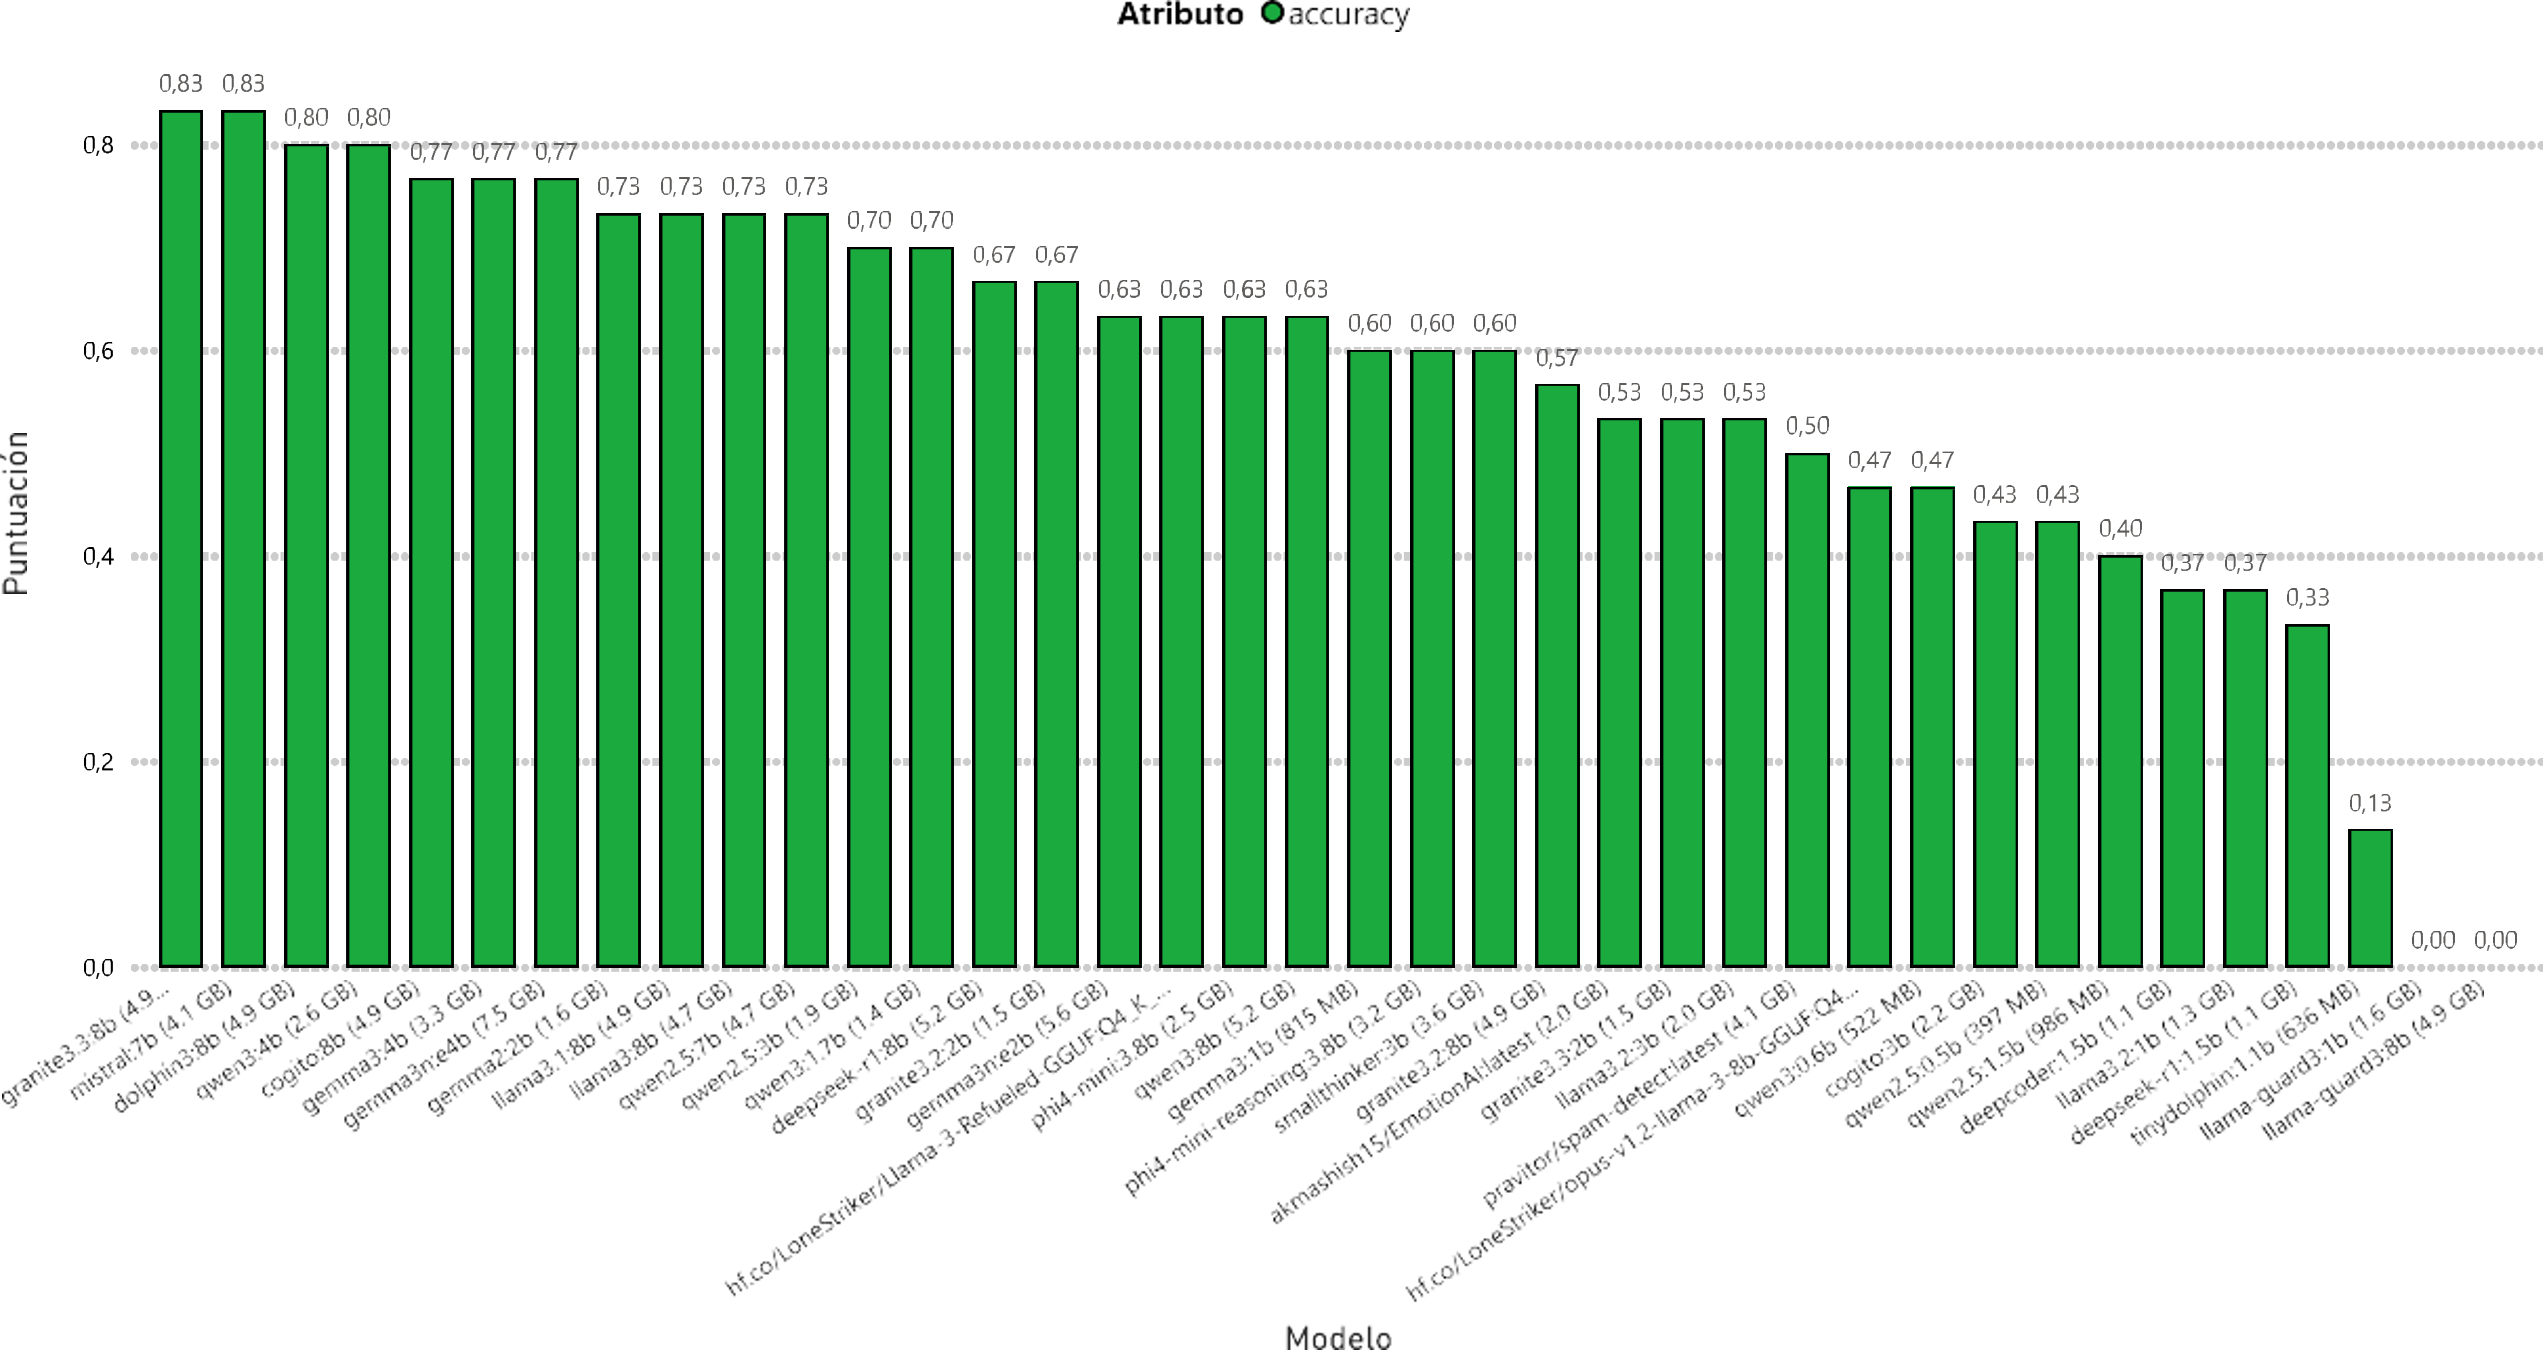
\includegraphics[width=1\linewidth]{imagenes/classificationTestsResults/Zero Shot Acurracy.png}
    \caption{Métrica de exactitud por cada modelo obtenida de las pruebas de identificación con la técnica de Zero Shot prompting}
    \label{fig:enter-label}
\end{figure}

\begin{figure}[H]
    \centering
    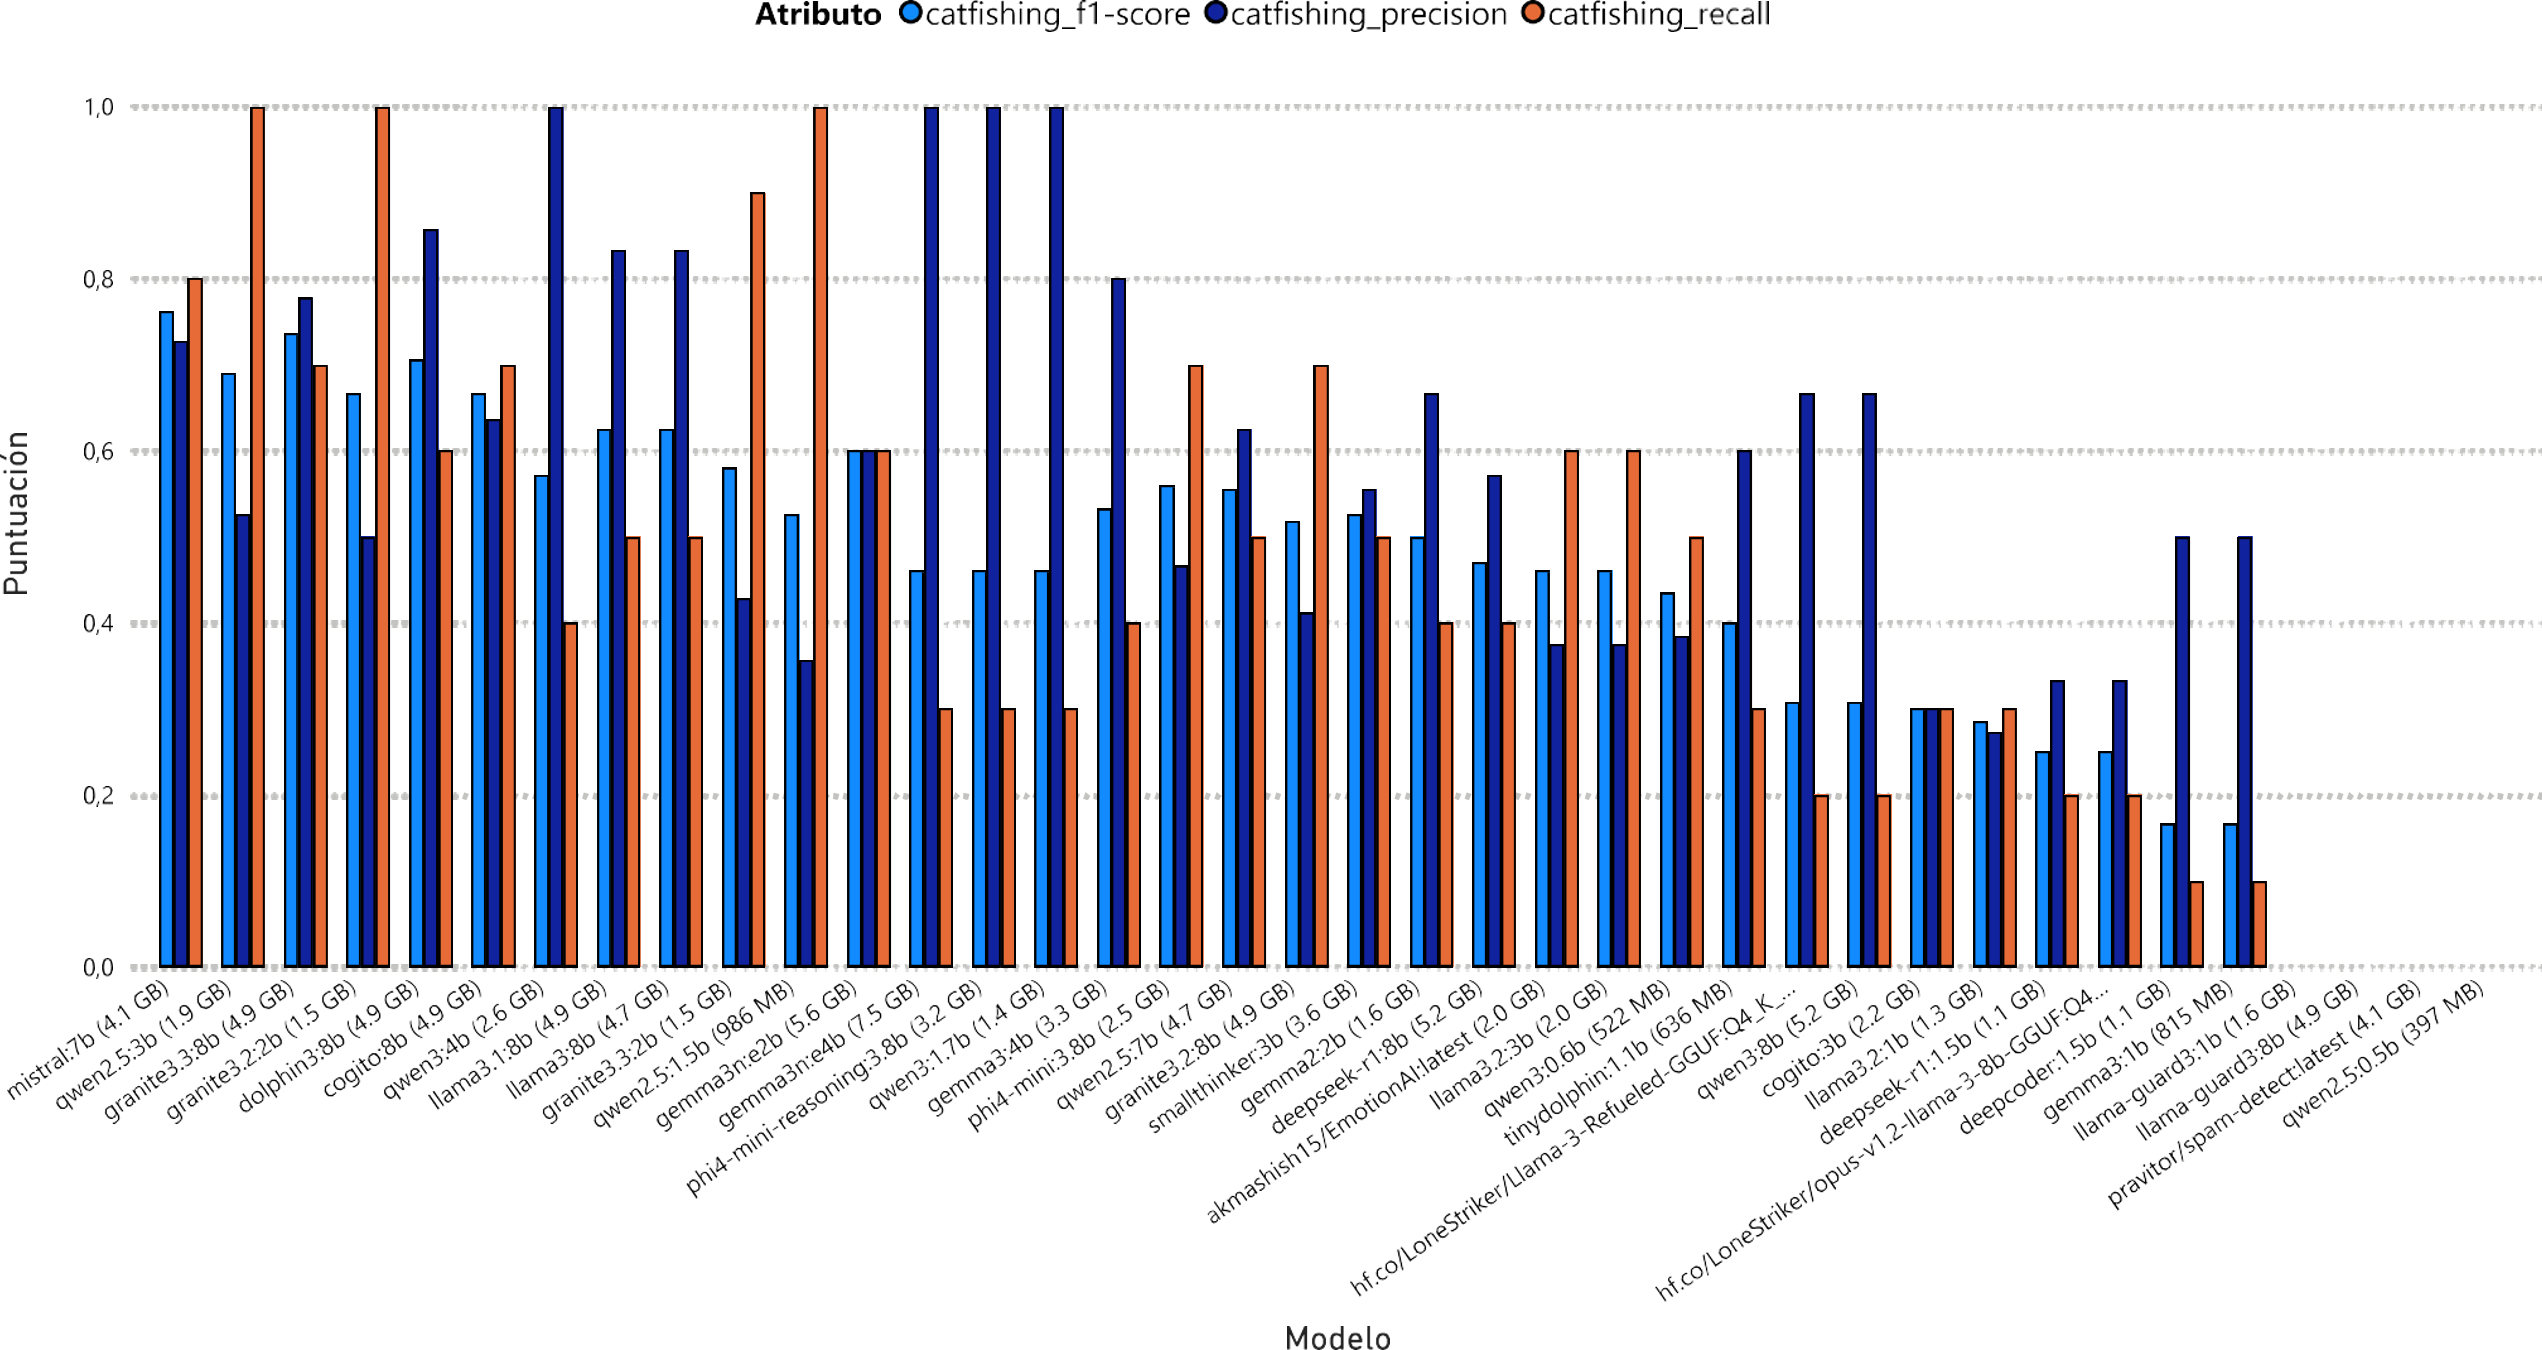
\includegraphics[width=1\linewidth]{imagenes/classificationTestsResults/Zero Shot Catfishing.png}
    \caption{Resultados de las pruebas de identificación de catfishing con la técnica Zero Shot prompting}
    \label{fig:zero-shot-catfishing}
\end{figure}

\begin{figure}[H]
    \centering
    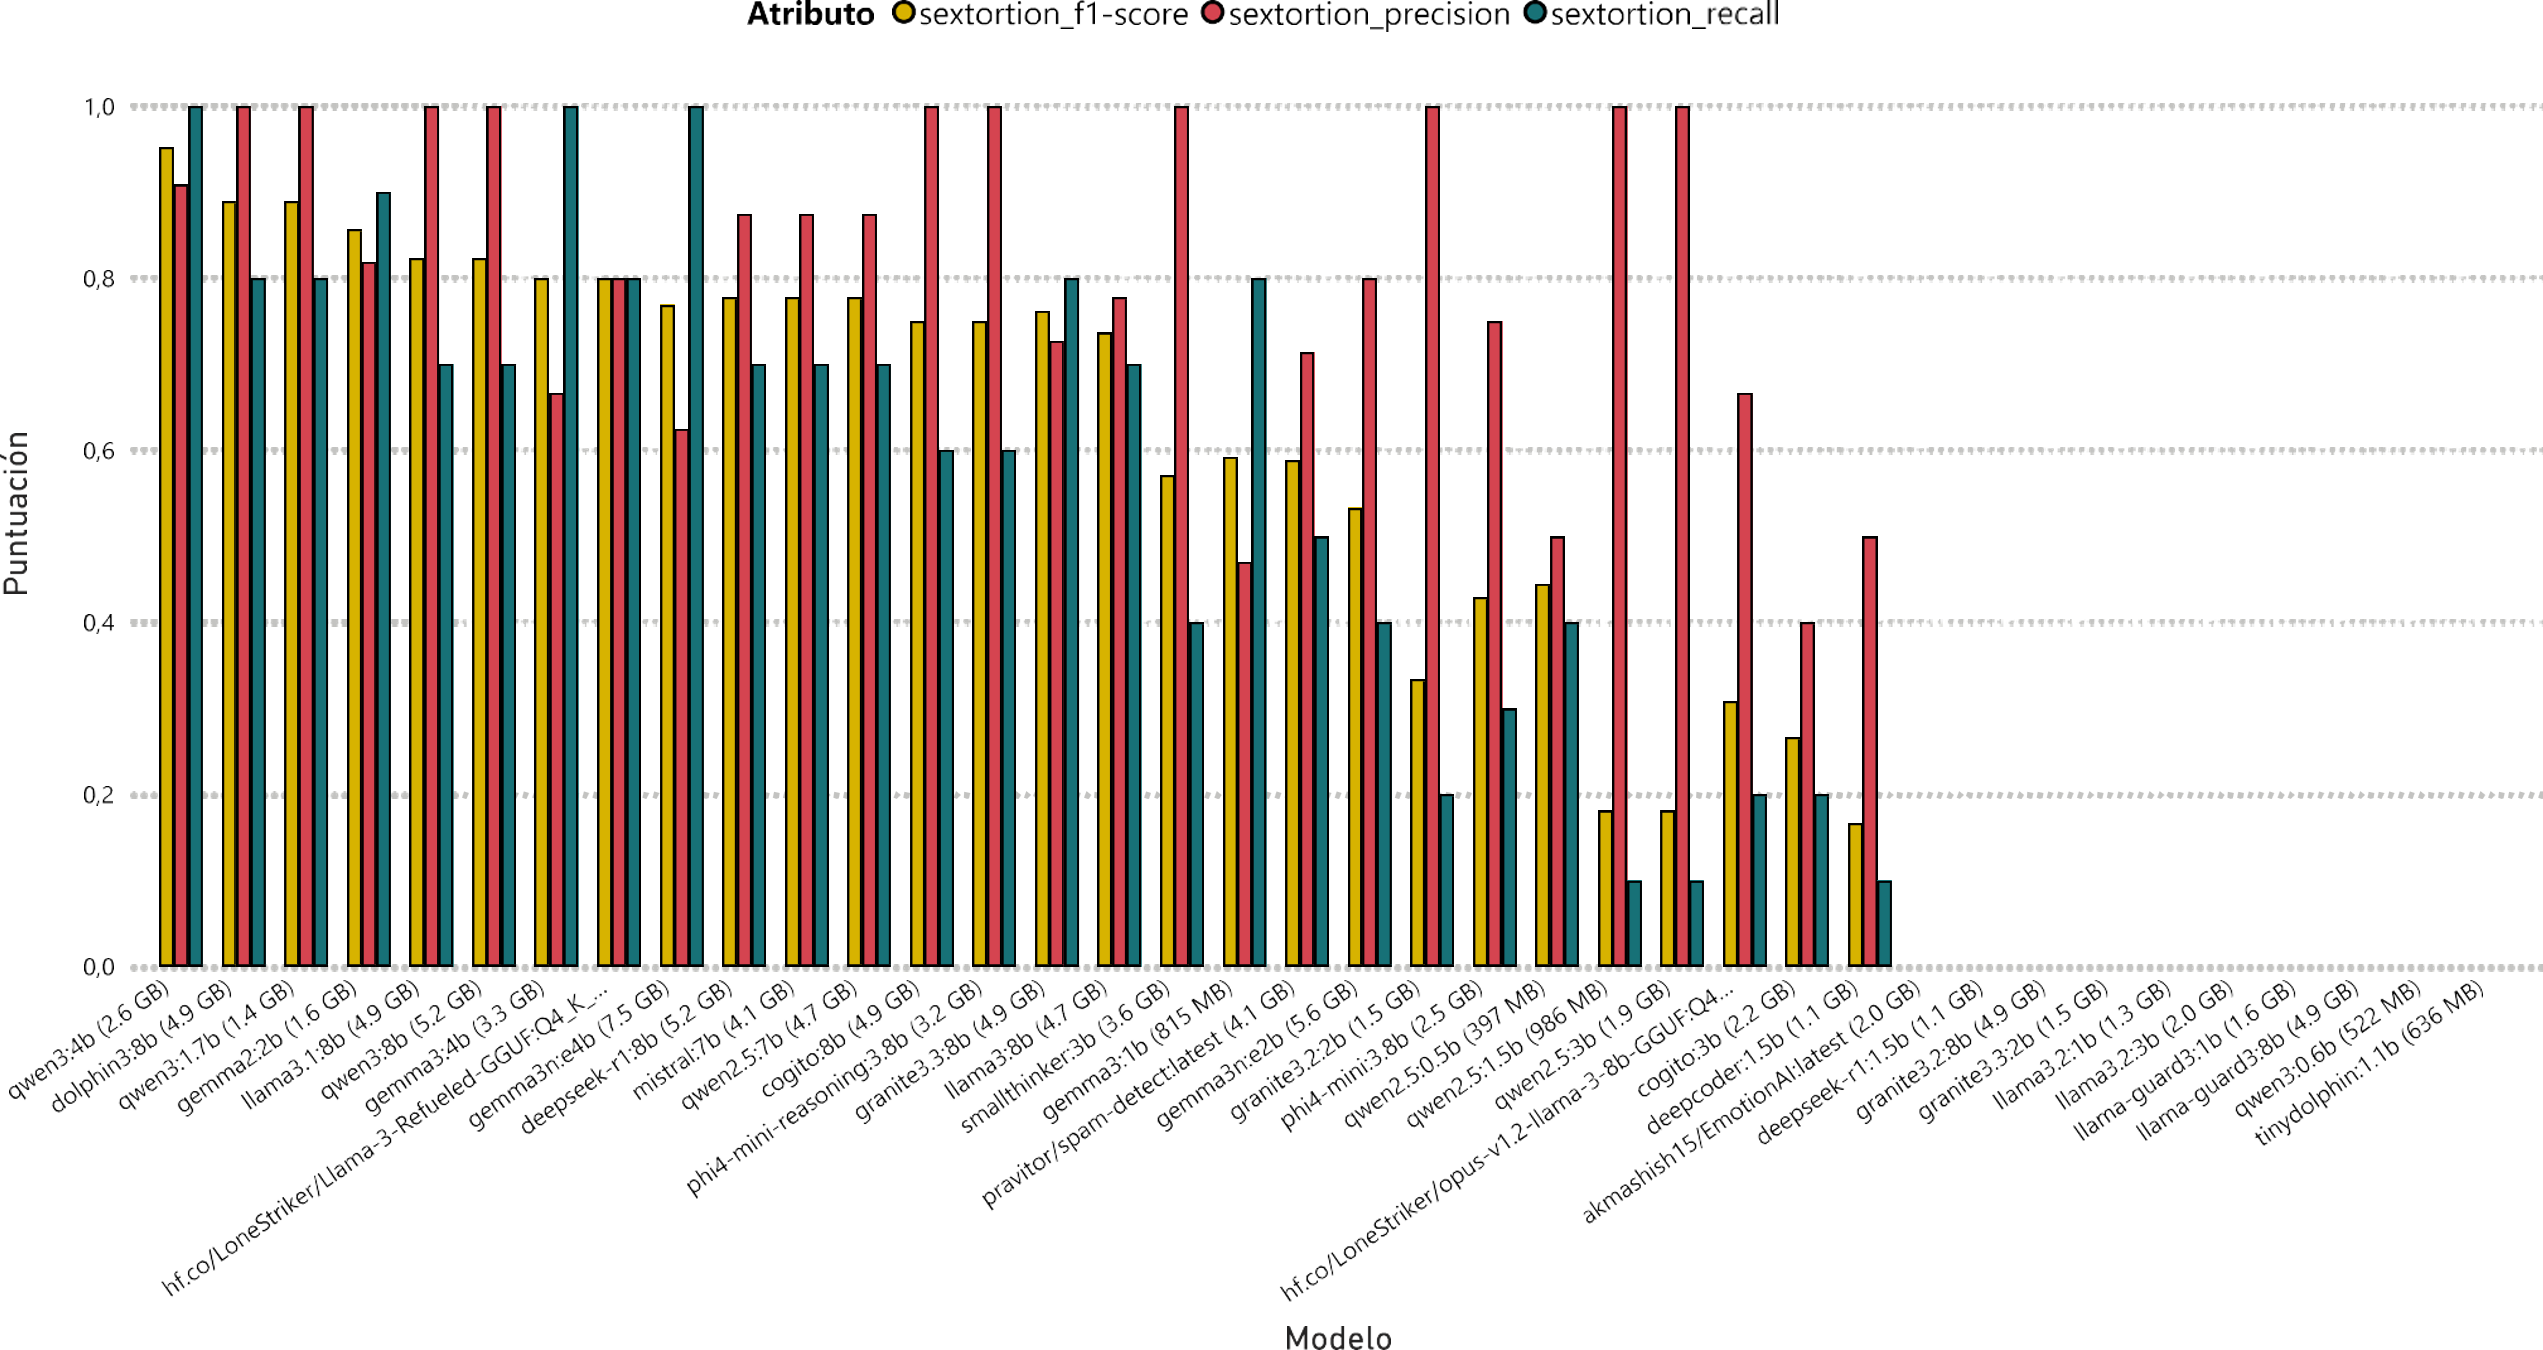
\includegraphics[width=1\linewidth]{imagenes/classificationTestsResults/Zero Shot Sextorción.png}
    \caption{Resultados de las pruebas de identificación de sextorción con la técnica Zero Shot prompting}
    \label{fig:zero-shot-sextorcion}
\end{figure}

\begin{figure}[H]
    \centering
    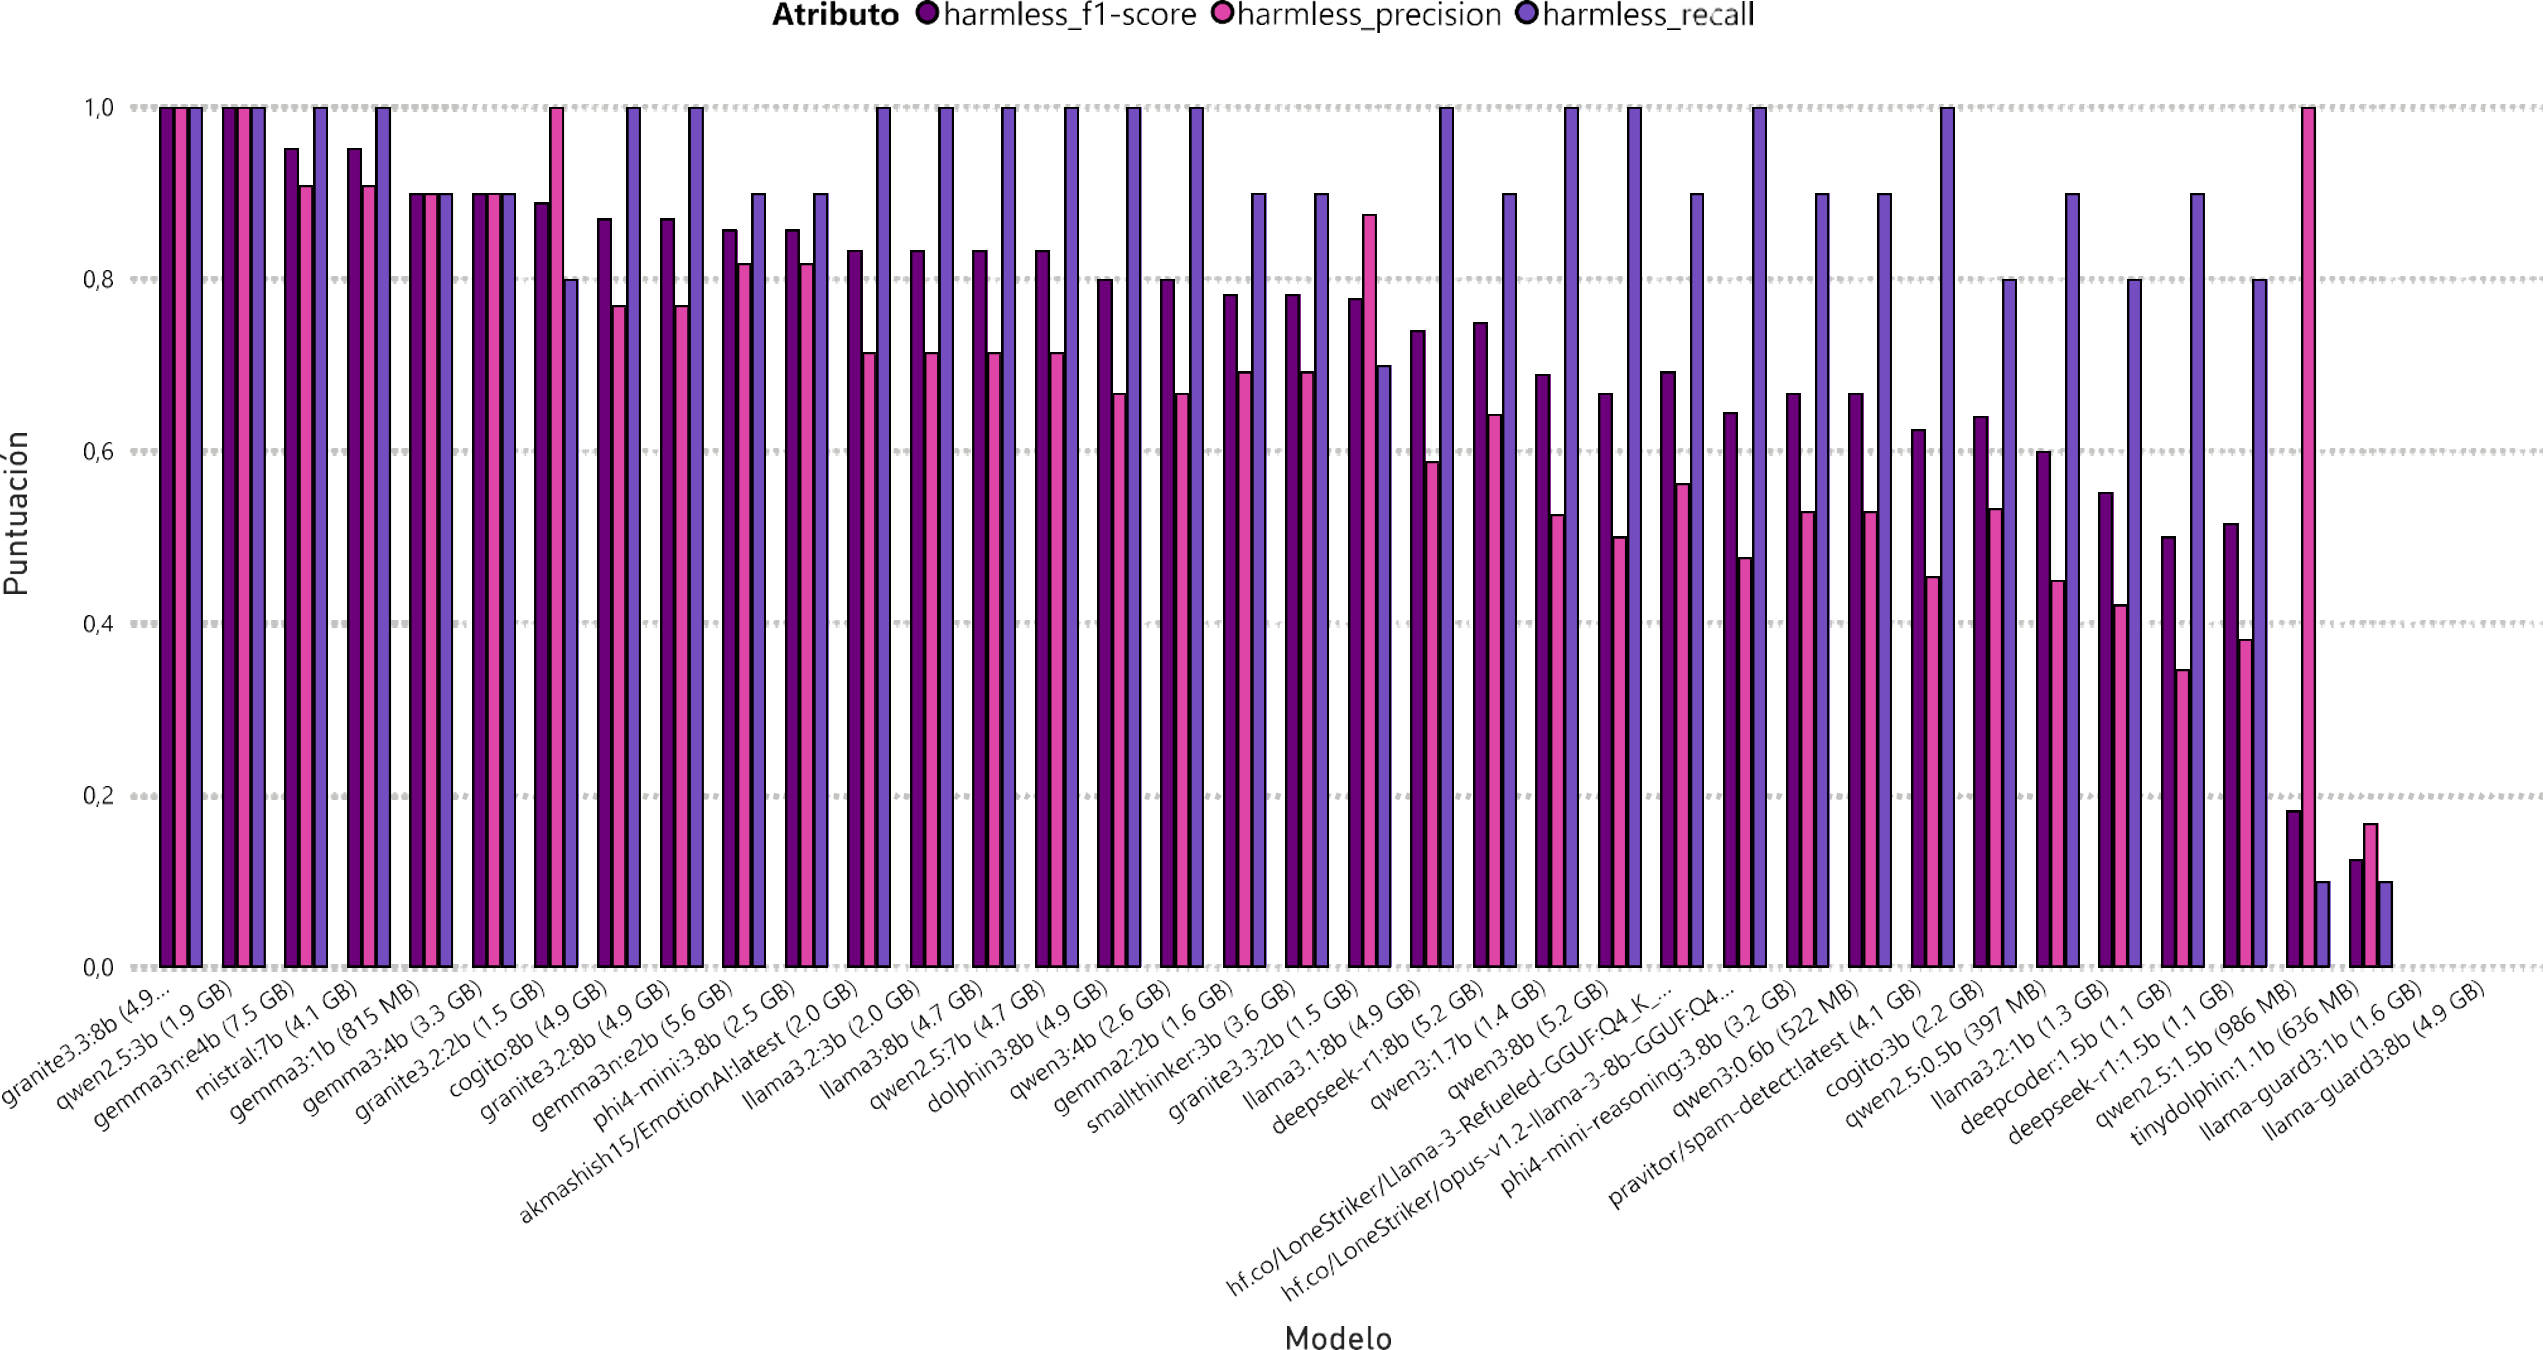
\includegraphics[width=1\linewidth]{imagenes/classificationTestsResults/Zero Shot Inofensivo.png}
    \caption{Resultados de las pruebas de identificación de inofensivo con la técnica Zero Shot prompting}
    \label{fig:zero-shot-inofensivo}
\end{figure}

% Resultados con Few Shot Prompting (Datos Sintéticos)

\begin{figure}[H]
    \centering
    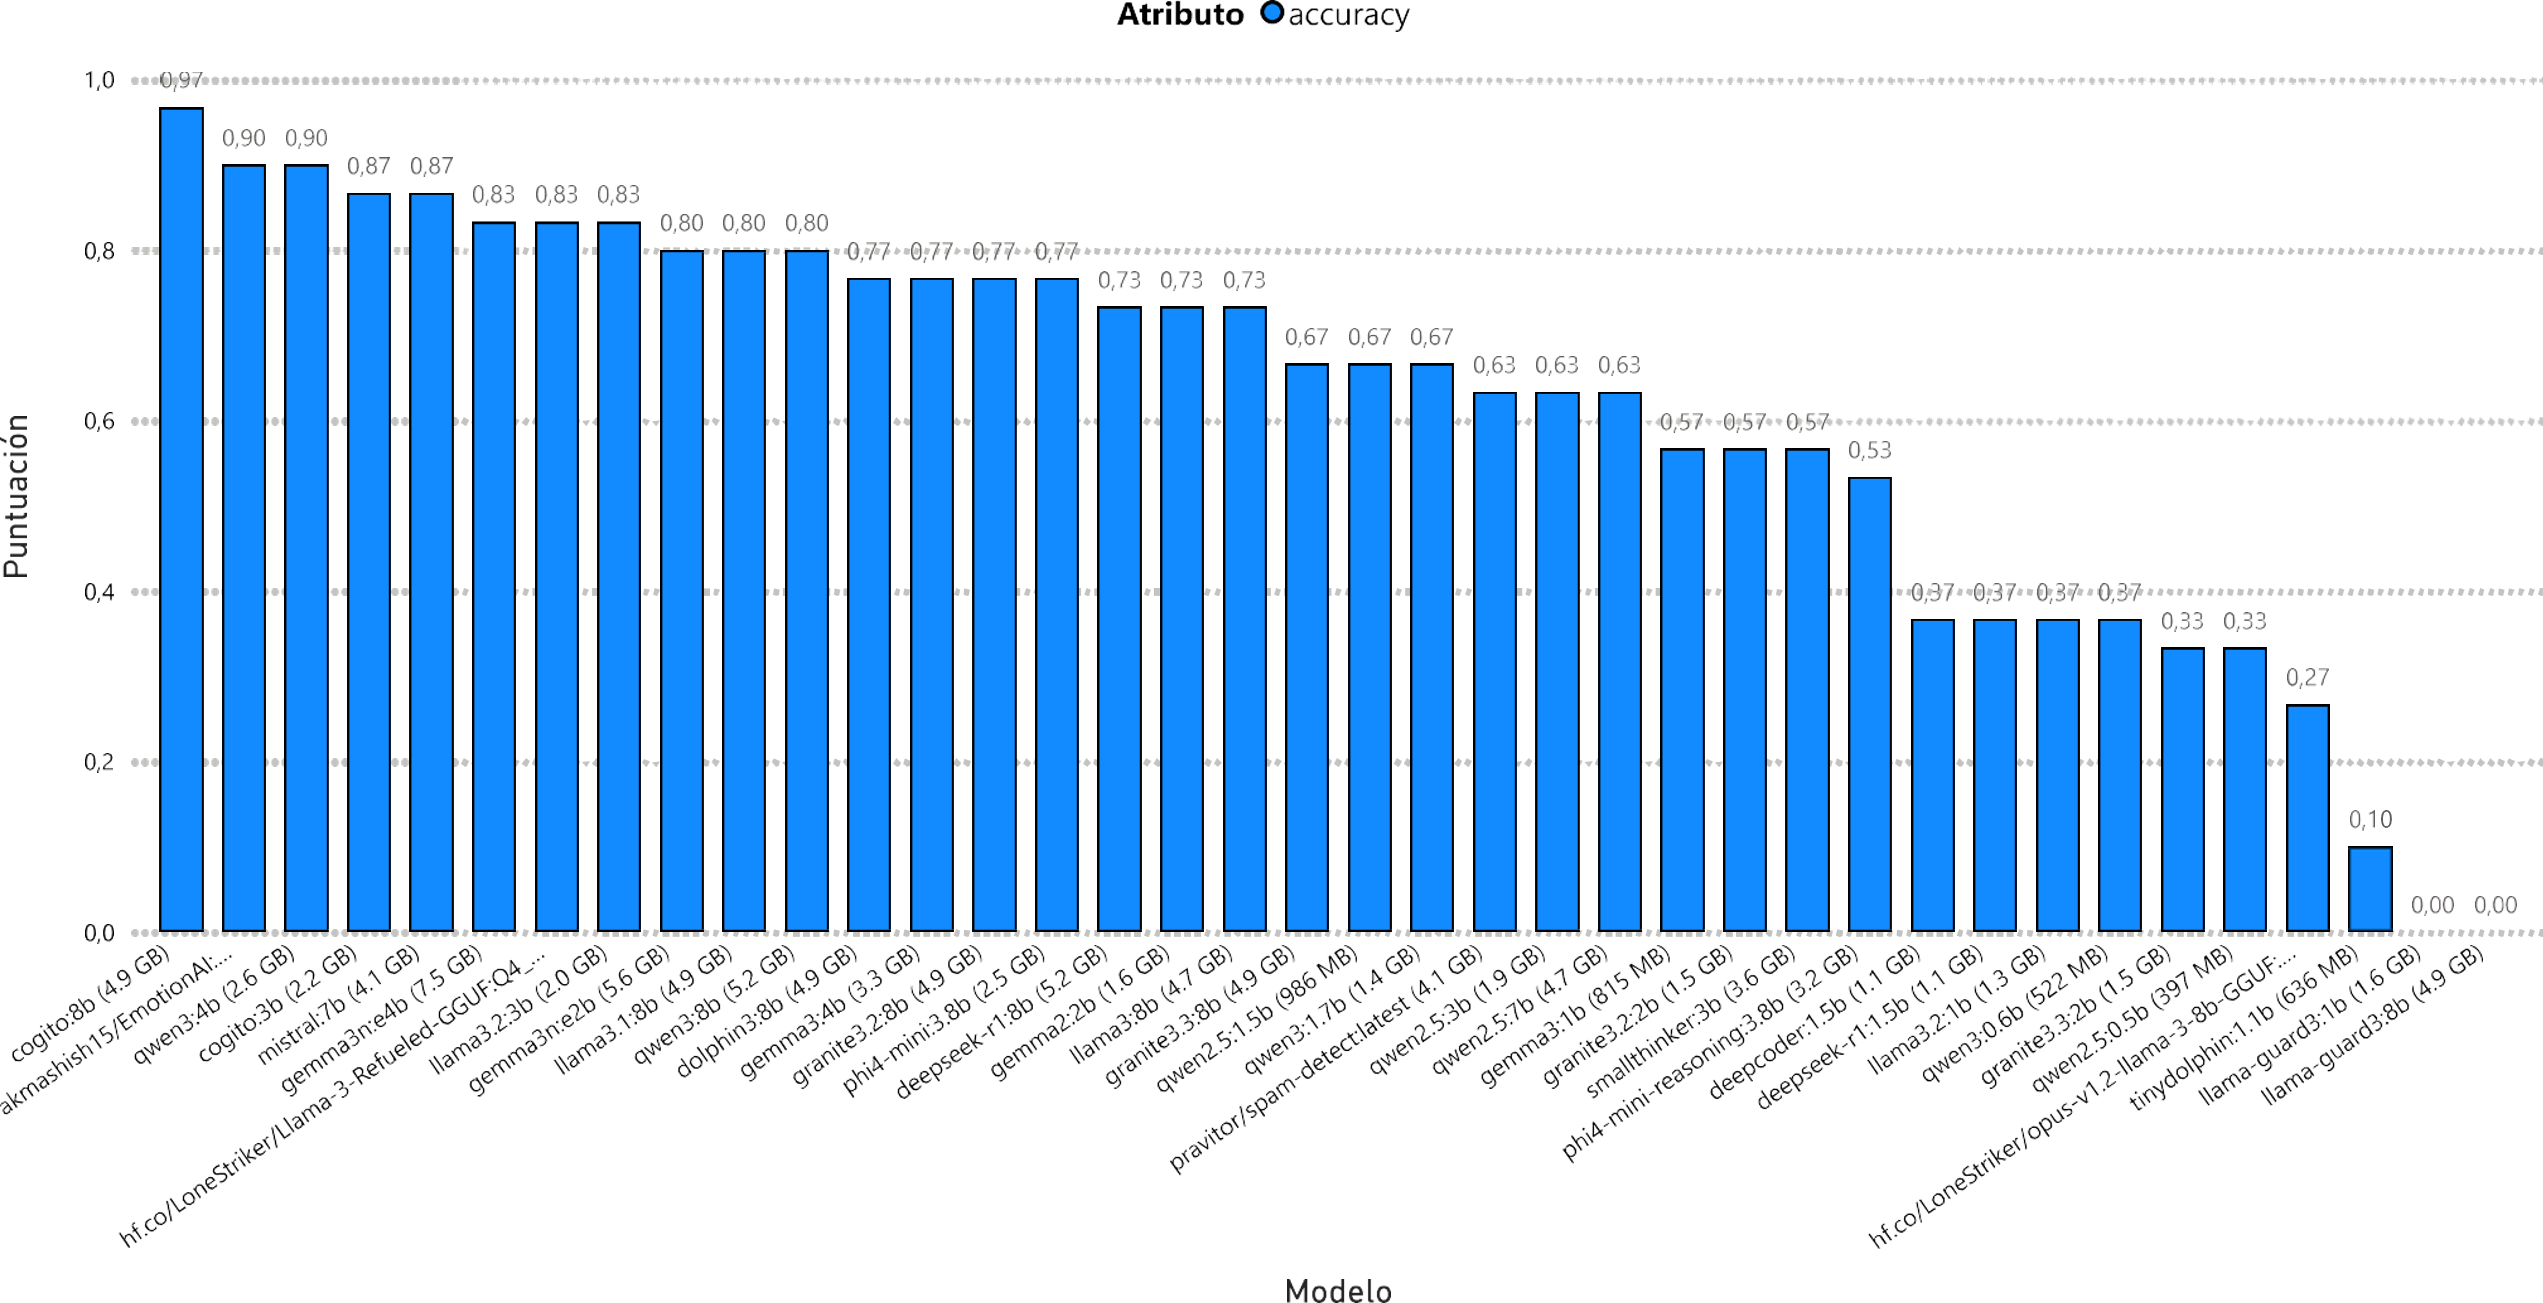
\includegraphics[width=1\linewidth]{imagenes/classificationTestsResults/Few Shot Sintético Acurracy.png}
    \caption{Métrica de exactitud por cada modelo obtenida de las pruebas de identificación con la técnica de Few Shot prompting a partir de un data set de refinamiento construido con datos sintéticos}
    \label{fig:few-shot-sintetico-accuracy}
\end{figure}

\begin{figure}[H]
    \centering
    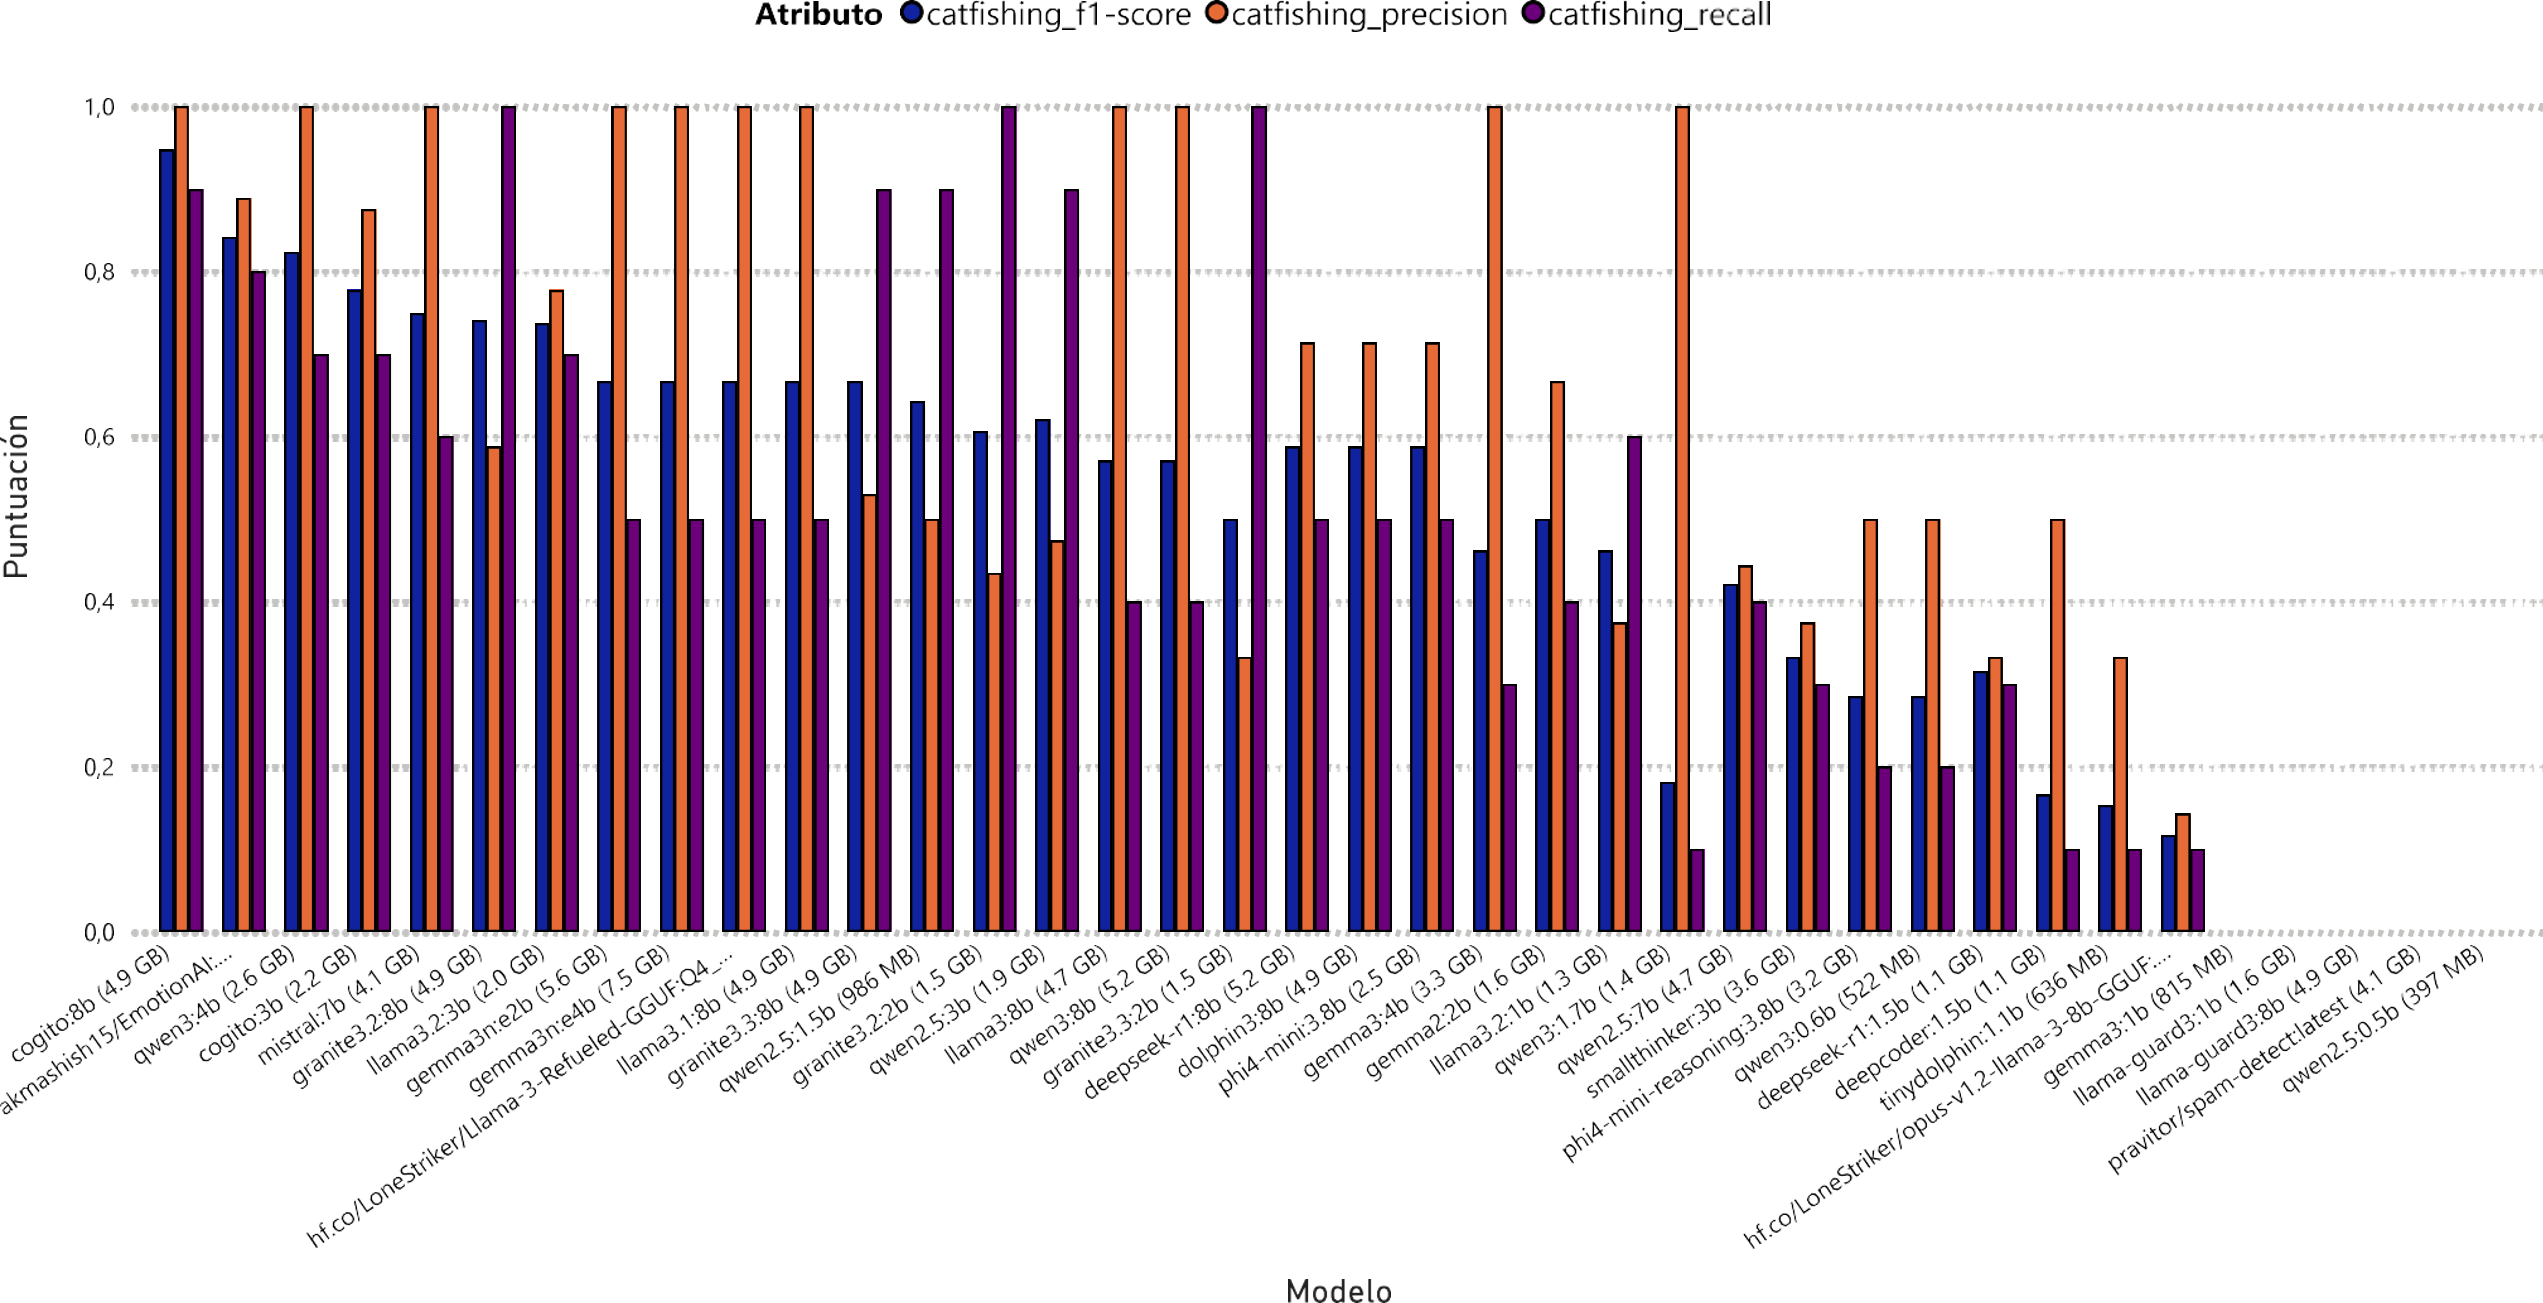
\includegraphics[width=1\linewidth]{imagenes/classificationTestsResults/Few Shot Sintético Catfishing.png}
    \caption{Resultados de las pruebas de identificación de catfishing con la técnica Few Shot prompting a partir de un data set de refinamiento construido con datos sintéticos}
    \label{fig:few-shot-sintetico-catfishing}
\end{figure}

\begin{figure}[H]
    \centering
    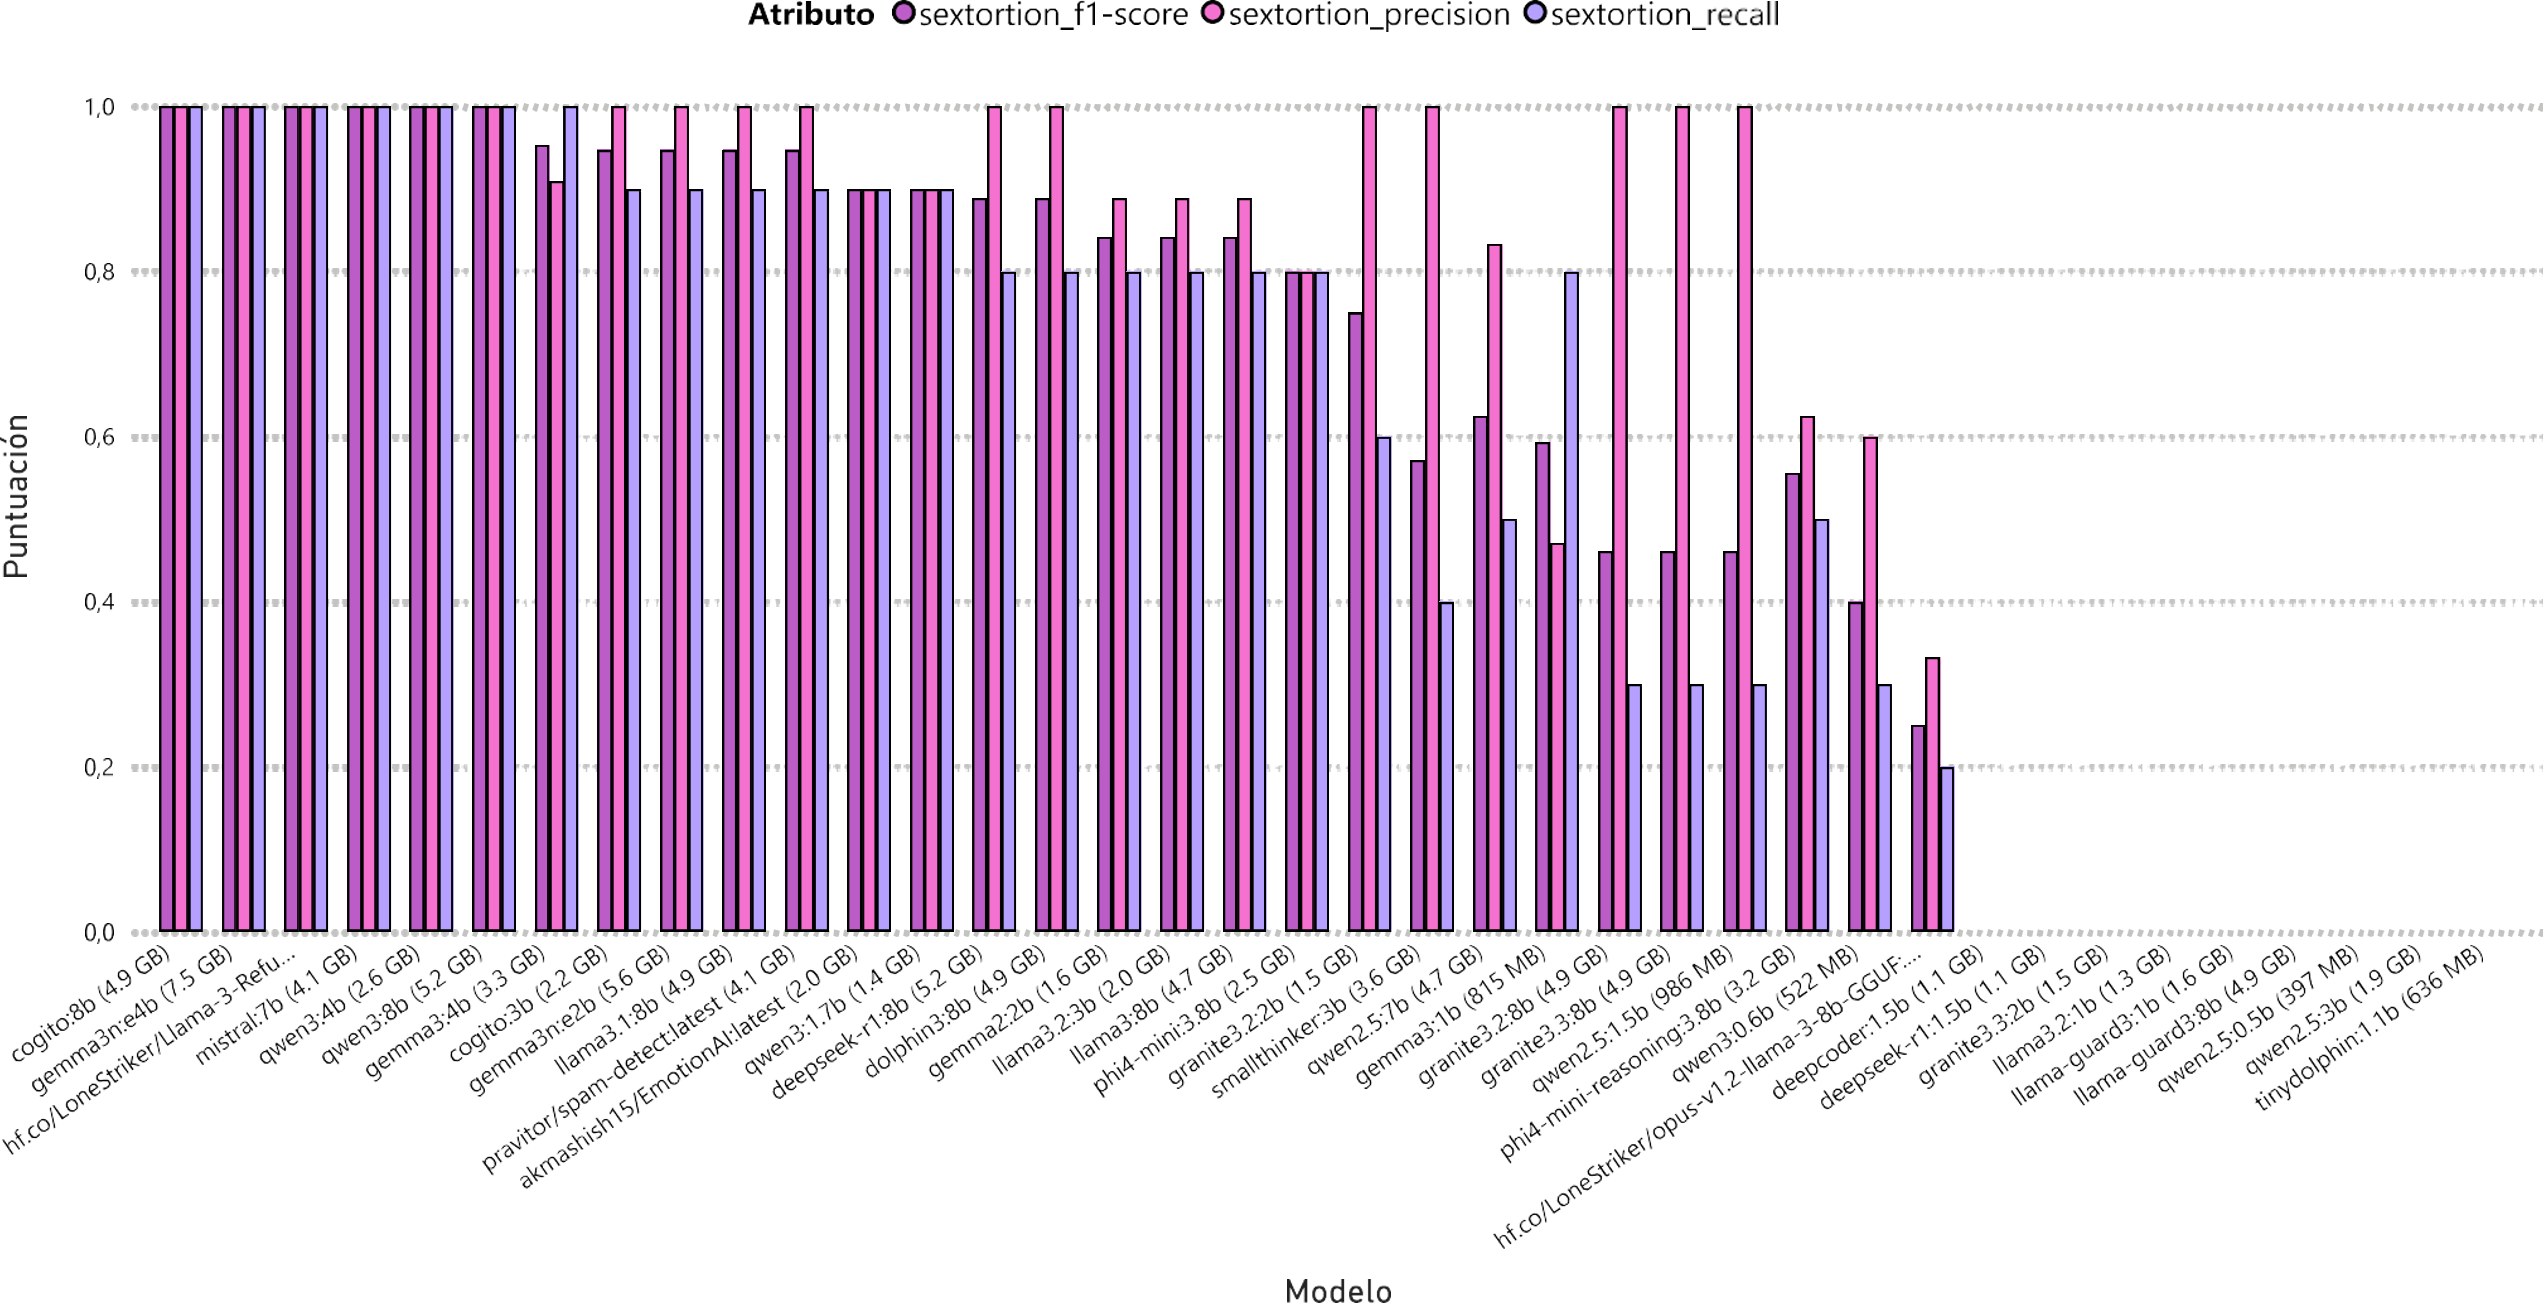
\includegraphics[width=1\linewidth]{imagenes/classificationTestsResults/Few Shot Sintético Sextorción.png}
    \caption{Resultados de las pruebas de identificación de sextorción con la técnica Few Shot prompting a partir de un data set de refinamiento construido con datos sintéticos}
    \label{fig:few-shot-sintetico-sextorcion}
\end{figure}

\begin{figure}[H]
    \centering
    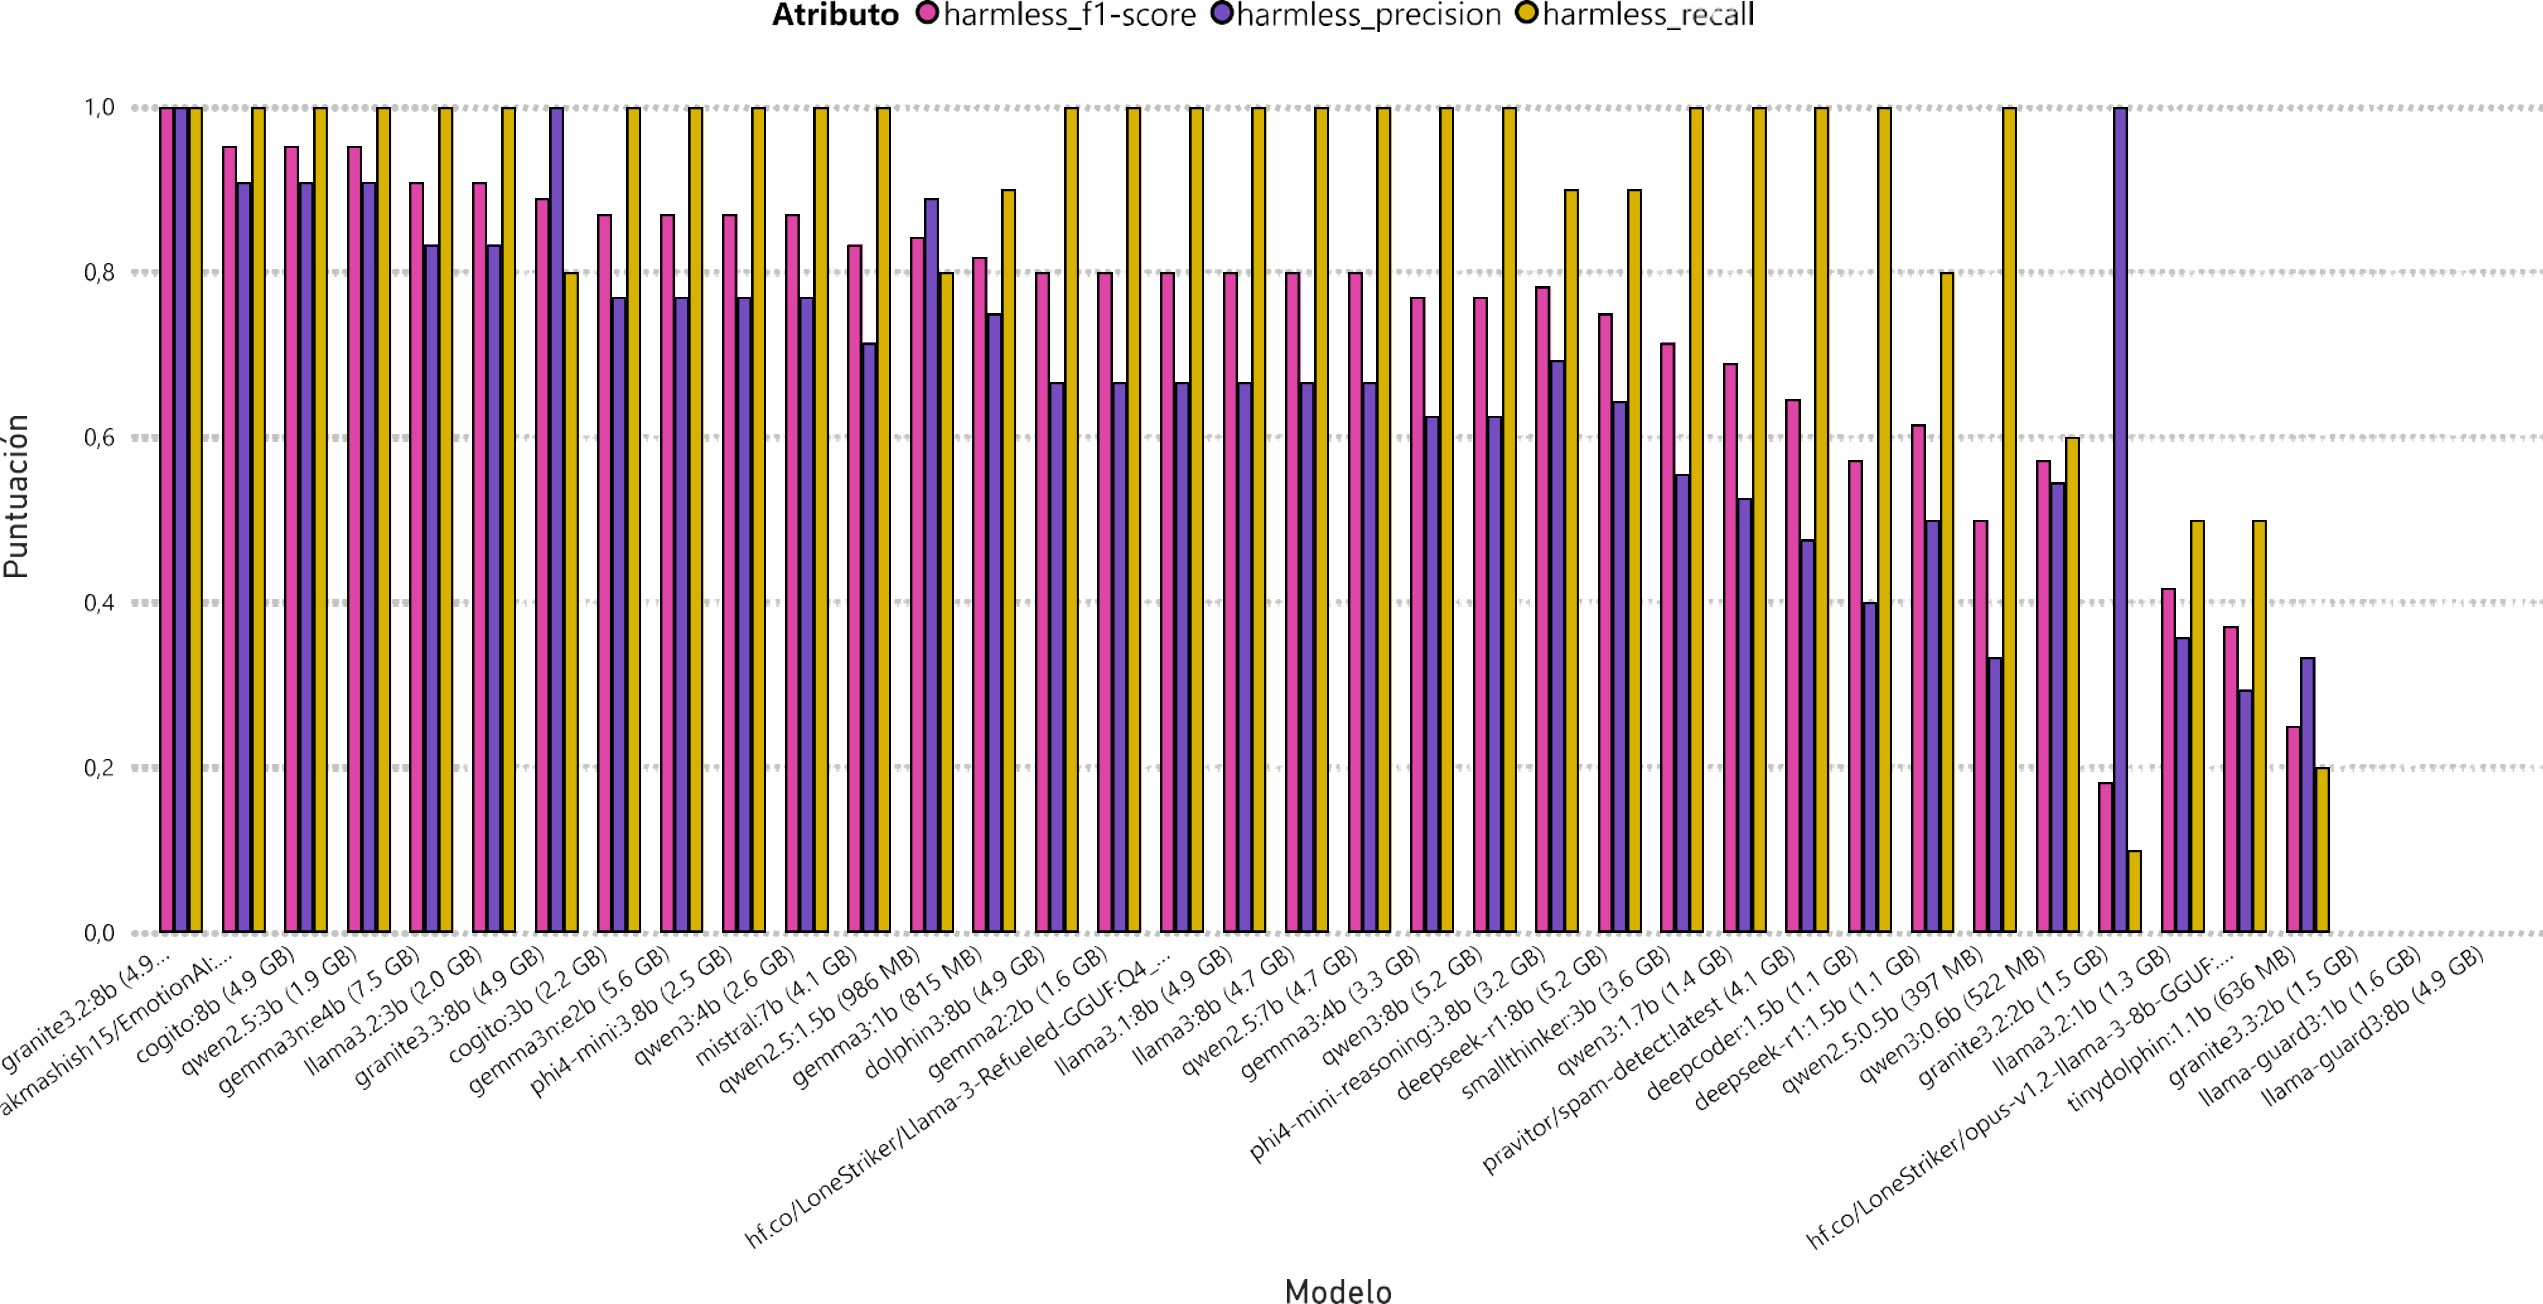
\includegraphics[width=1\linewidth]{imagenes/classificationTestsResults/Few Shot Sintético Inofensivo.png}
    \caption{Resultados de las pruebas de identificación de inofensivo con la técnica Few Shot prompting a partir de un data set de refinamiento construido con datos sintéticos}
    \label{fig:few-shot-sintetico-inofensivo}
\end{figure}

% Resultados con Few Shot Prompting (Datos Reales)

\begin{figure}[H]
    \centering
    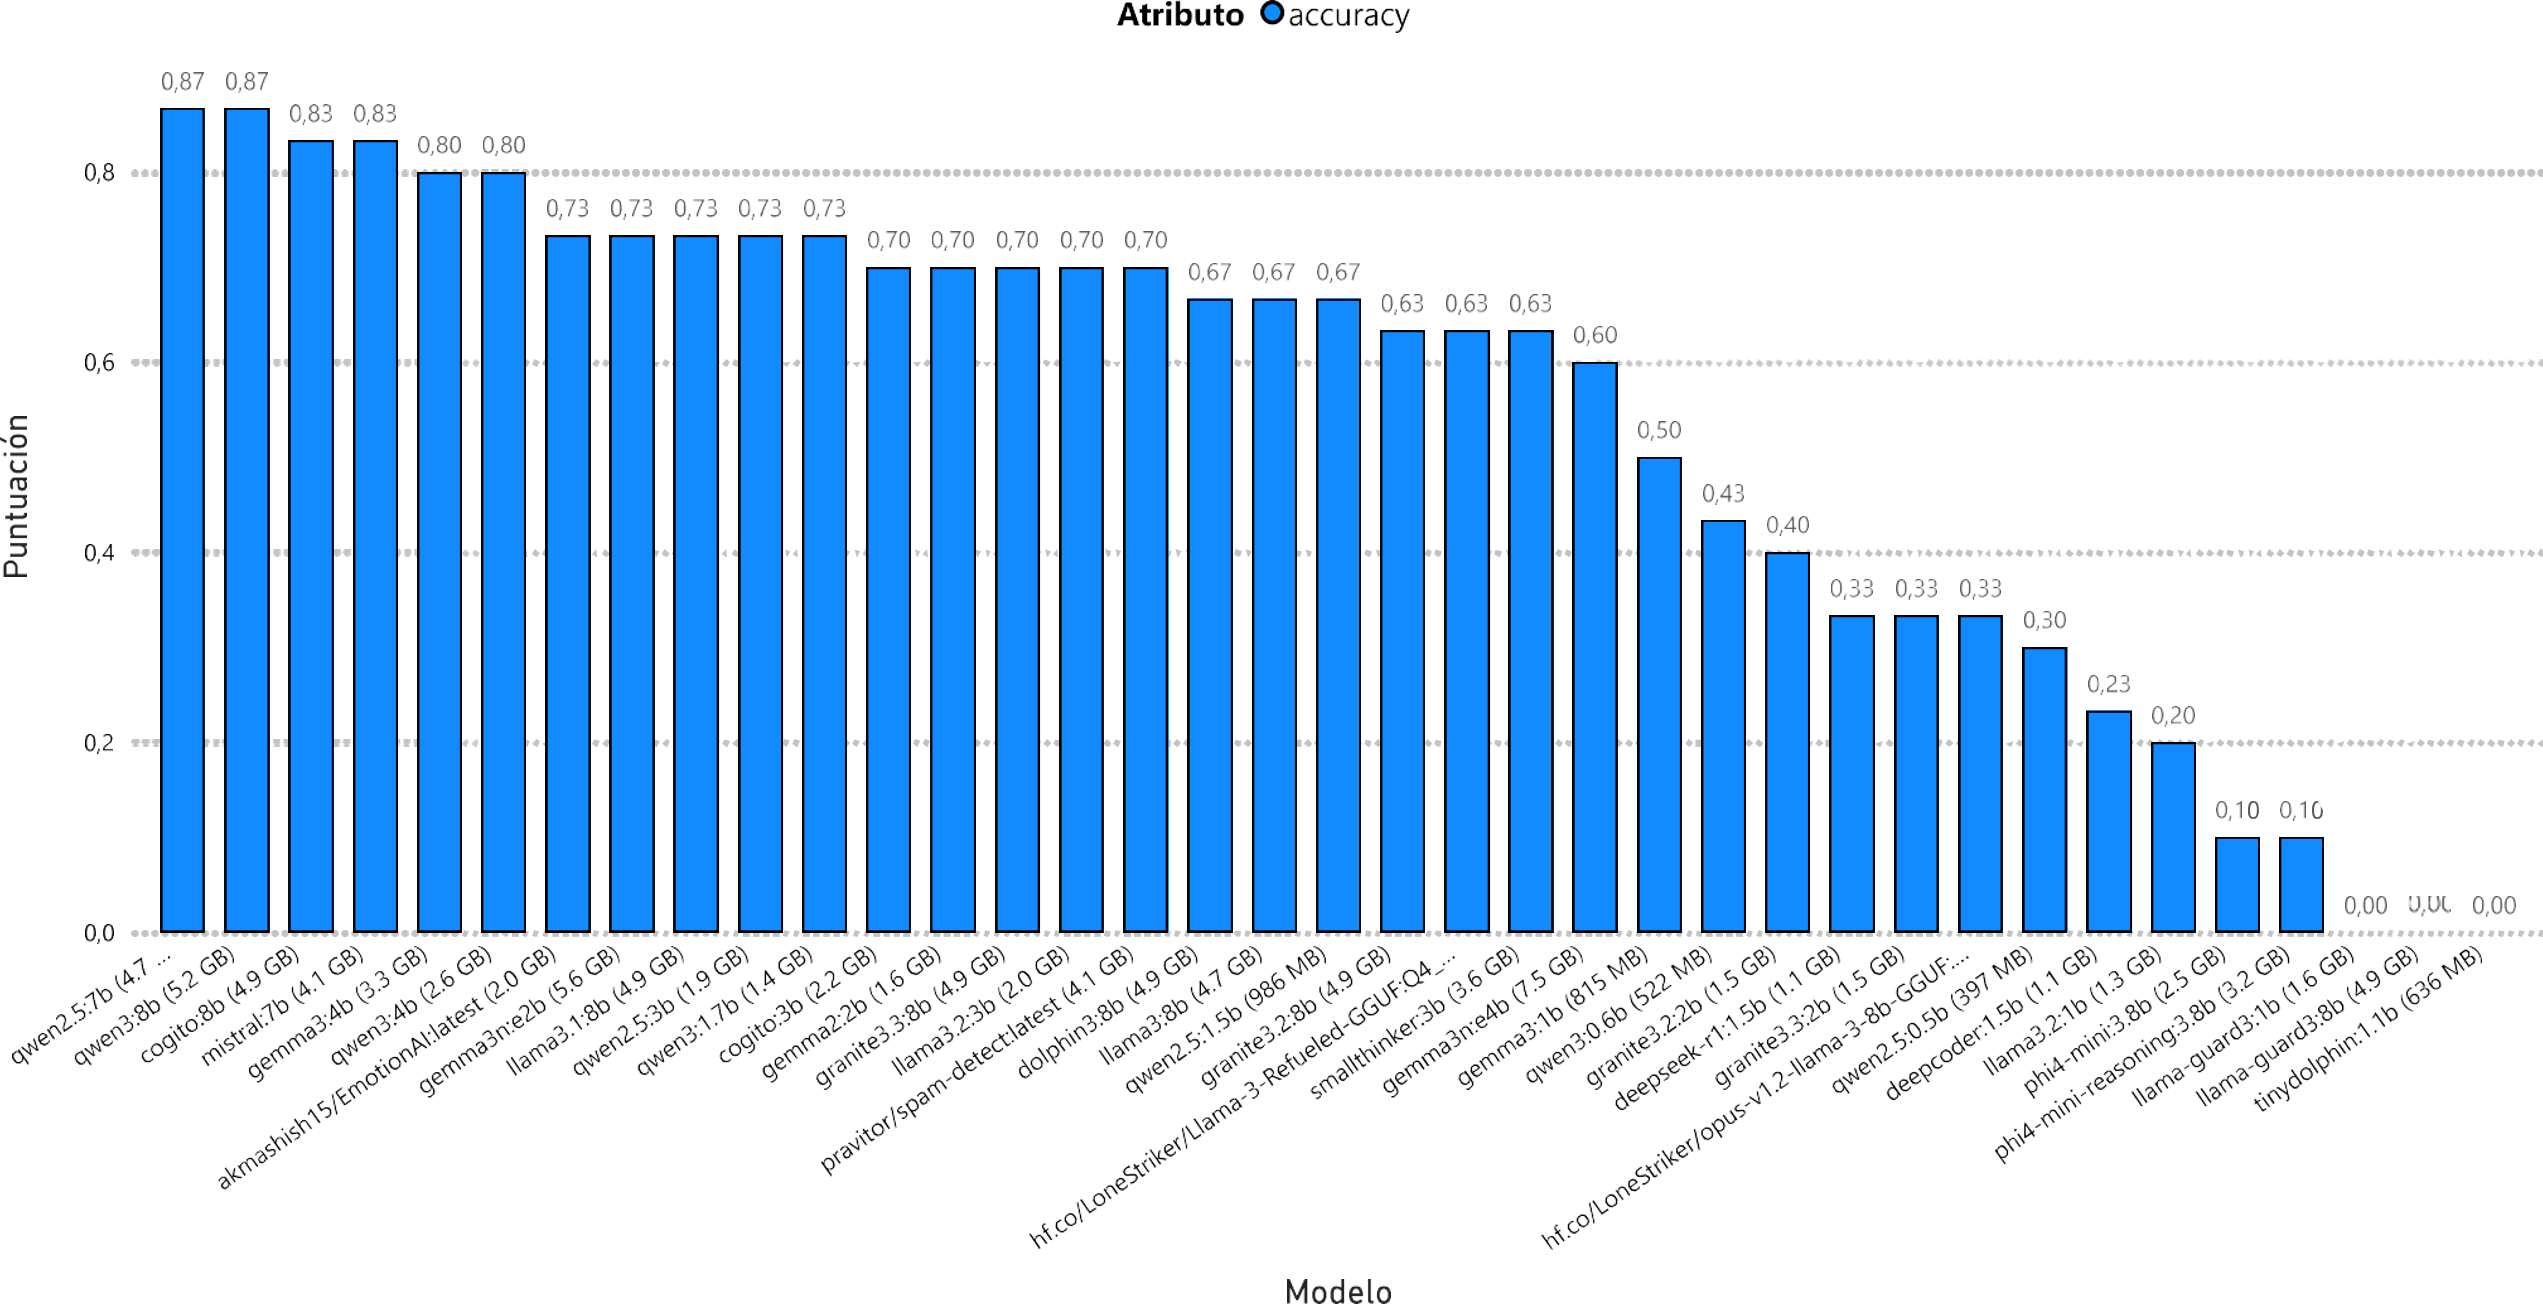
\includegraphics[width=1\linewidth]{imagenes/classificationTestsResults/Few Shot Real Acurracy.png}
    \caption{Métrica de exactitud por cada modelo obtenida de las pruebas de identificación con la técnica de Few Shot prompting a partir de un data set de refinamiento construido con datos reales}
    \label{fig:few-shot-real-accuracy}
\end{figure}

\begin{figure}[H]
    \centering
    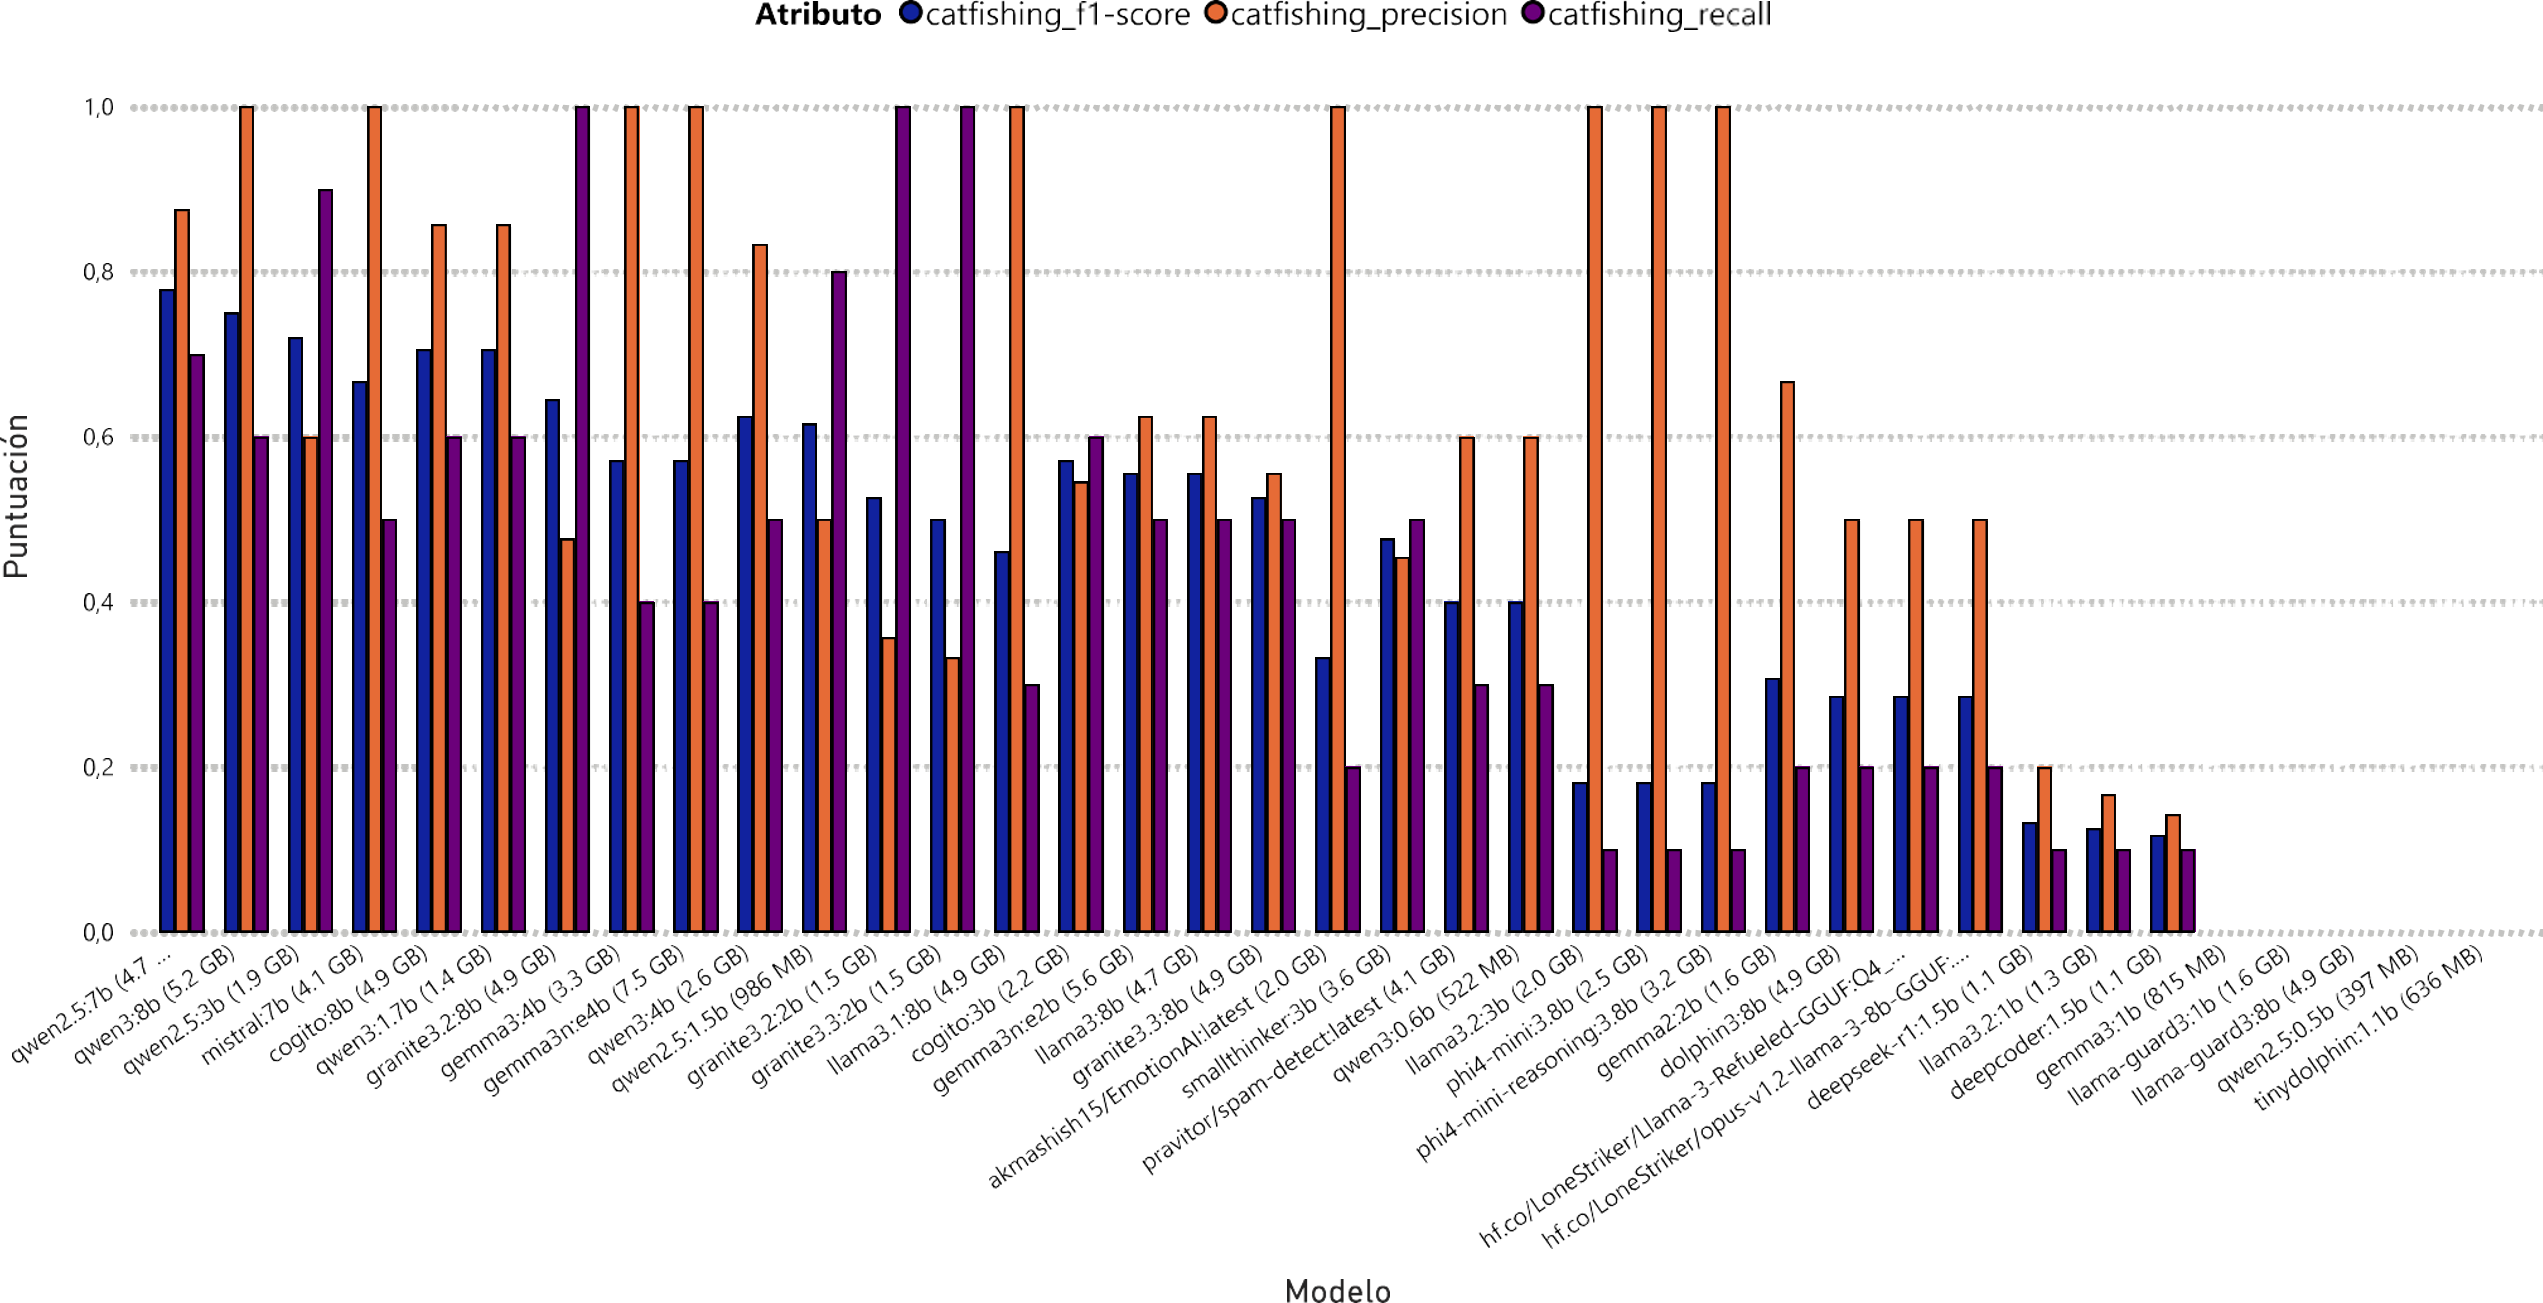
\includegraphics[width=1\linewidth]{imagenes/classificationTestsResults/Few Shot Real Catfishing.png}
    \caption{Resultados de las pruebas de identificación de catfishing con la técnica Few Shot prompting a partir de un data set de refinamiento construido con datos reales}
    \label{fig:few-shot-real-catfishing}
\end{figure}

\begin{figure}[H]
    \centering
    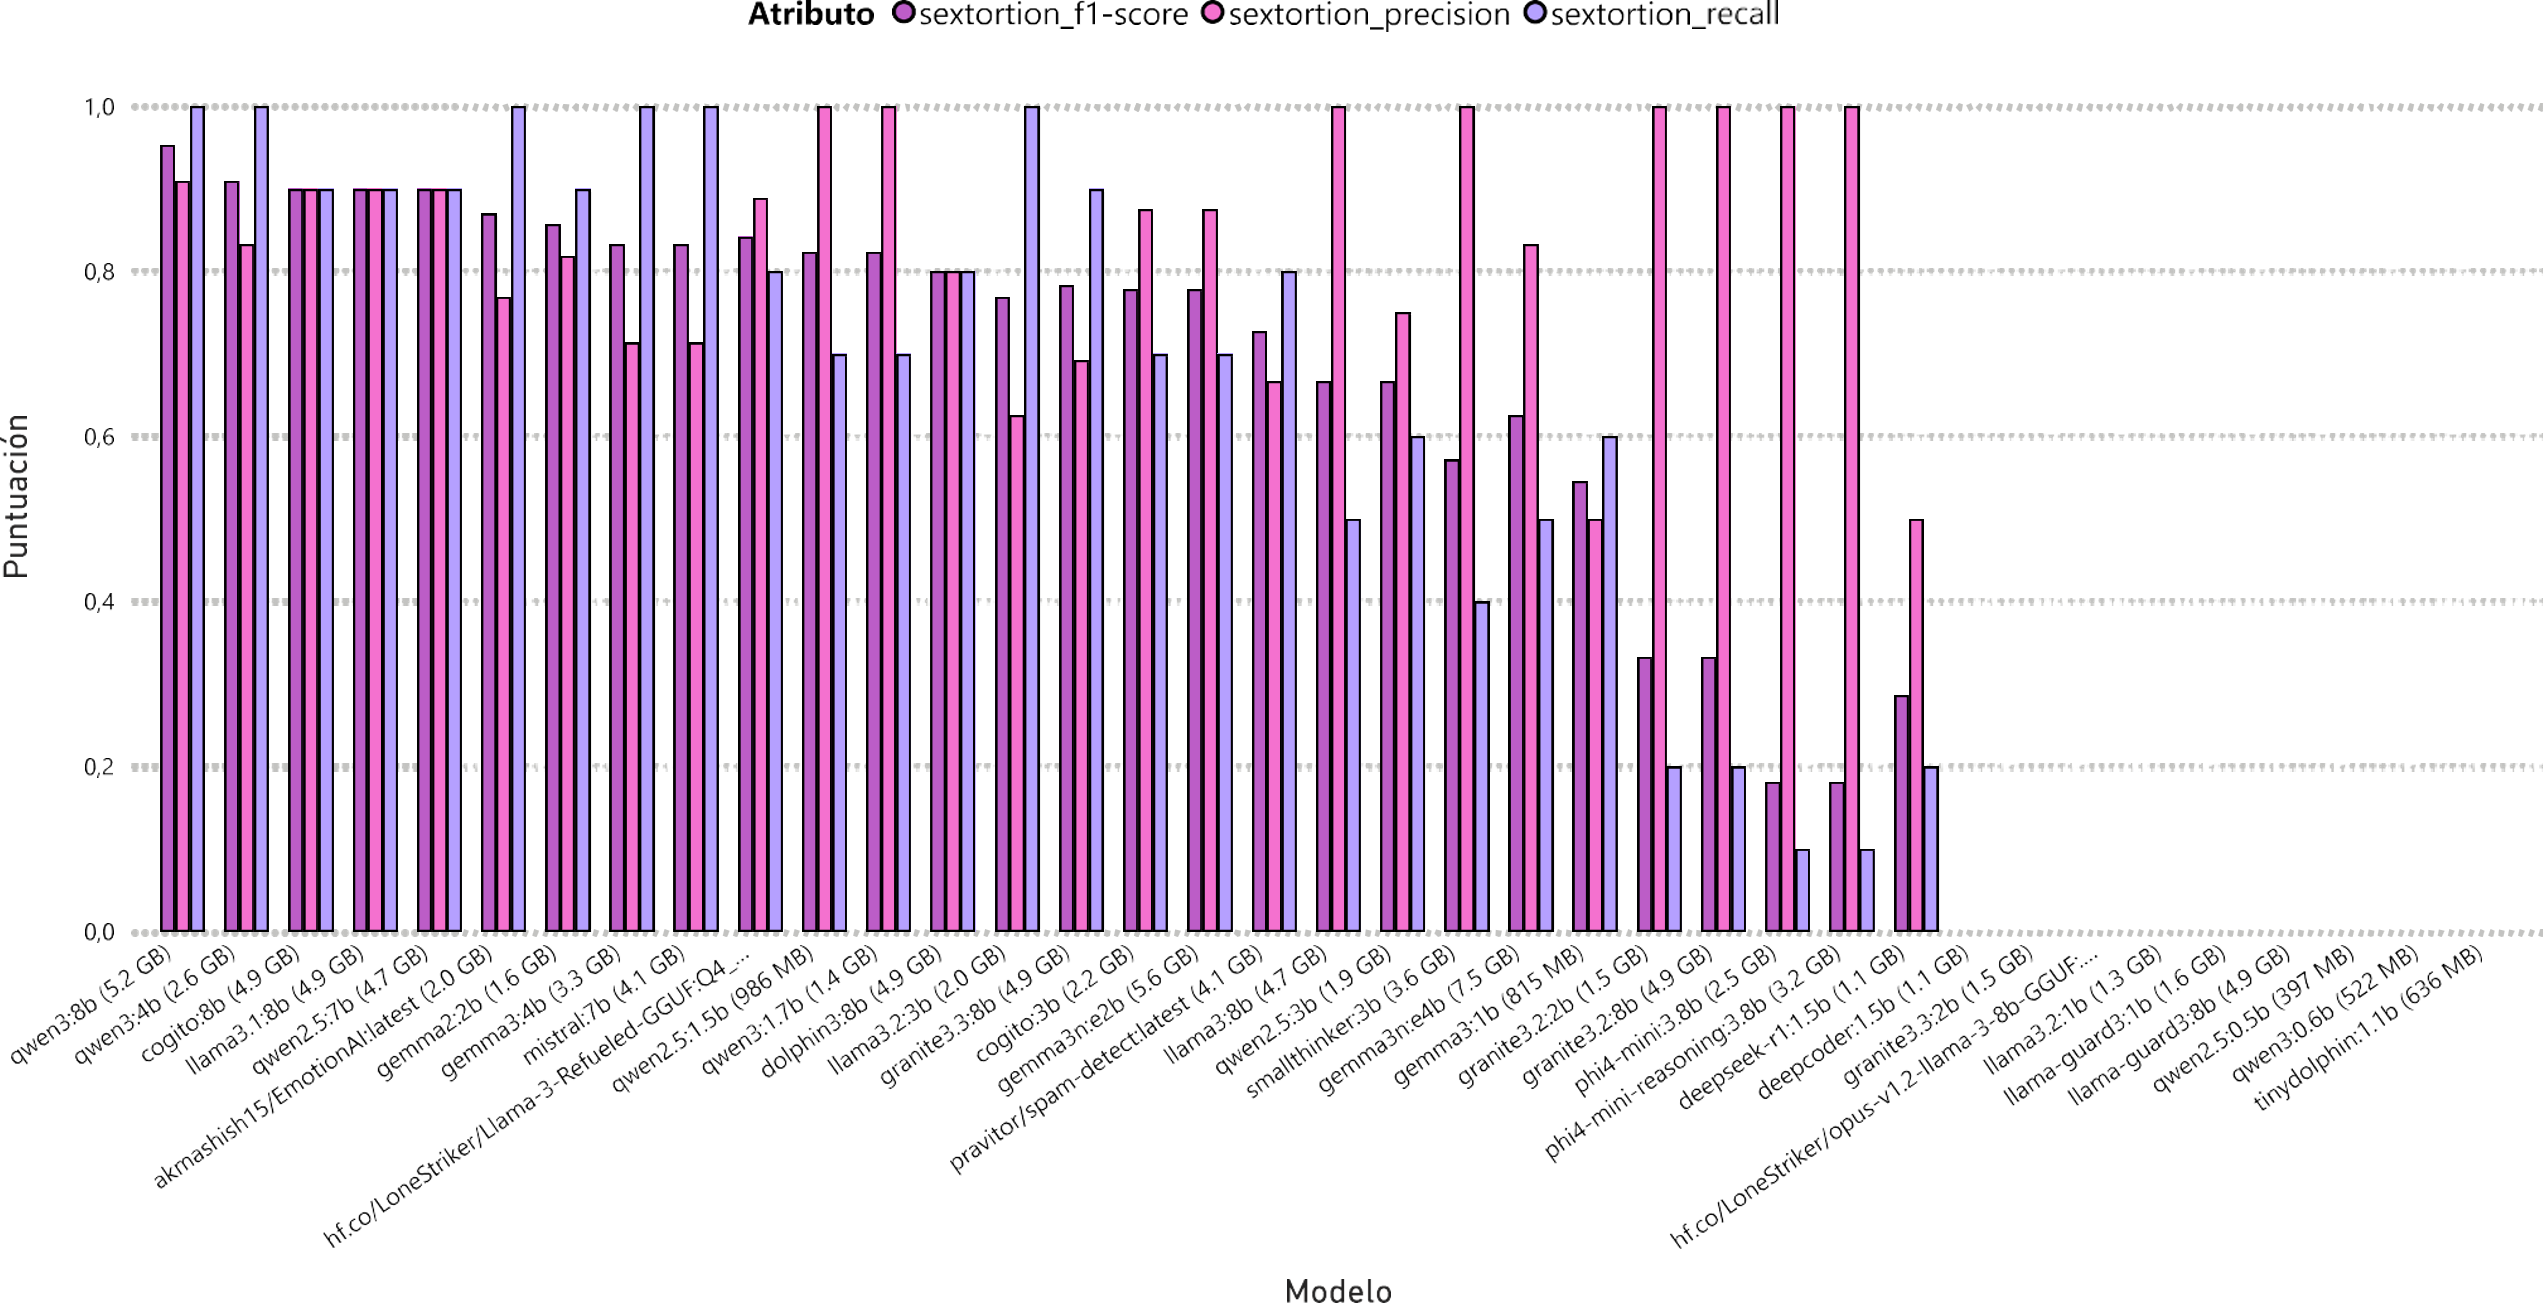
\includegraphics[width=1\linewidth]{imagenes/classificationTestsResults/Few Shot Real Sextorción.png}
    \caption{Resultados de las pruebas de identificación de sextorción con la técnica Few Shot prompting a partir de un data set de refinamiento construido con datos reales}
    \label{fig:few-shot-real-sextorcion}
\end{figure}

\begin{figure}[H]
    \centering
    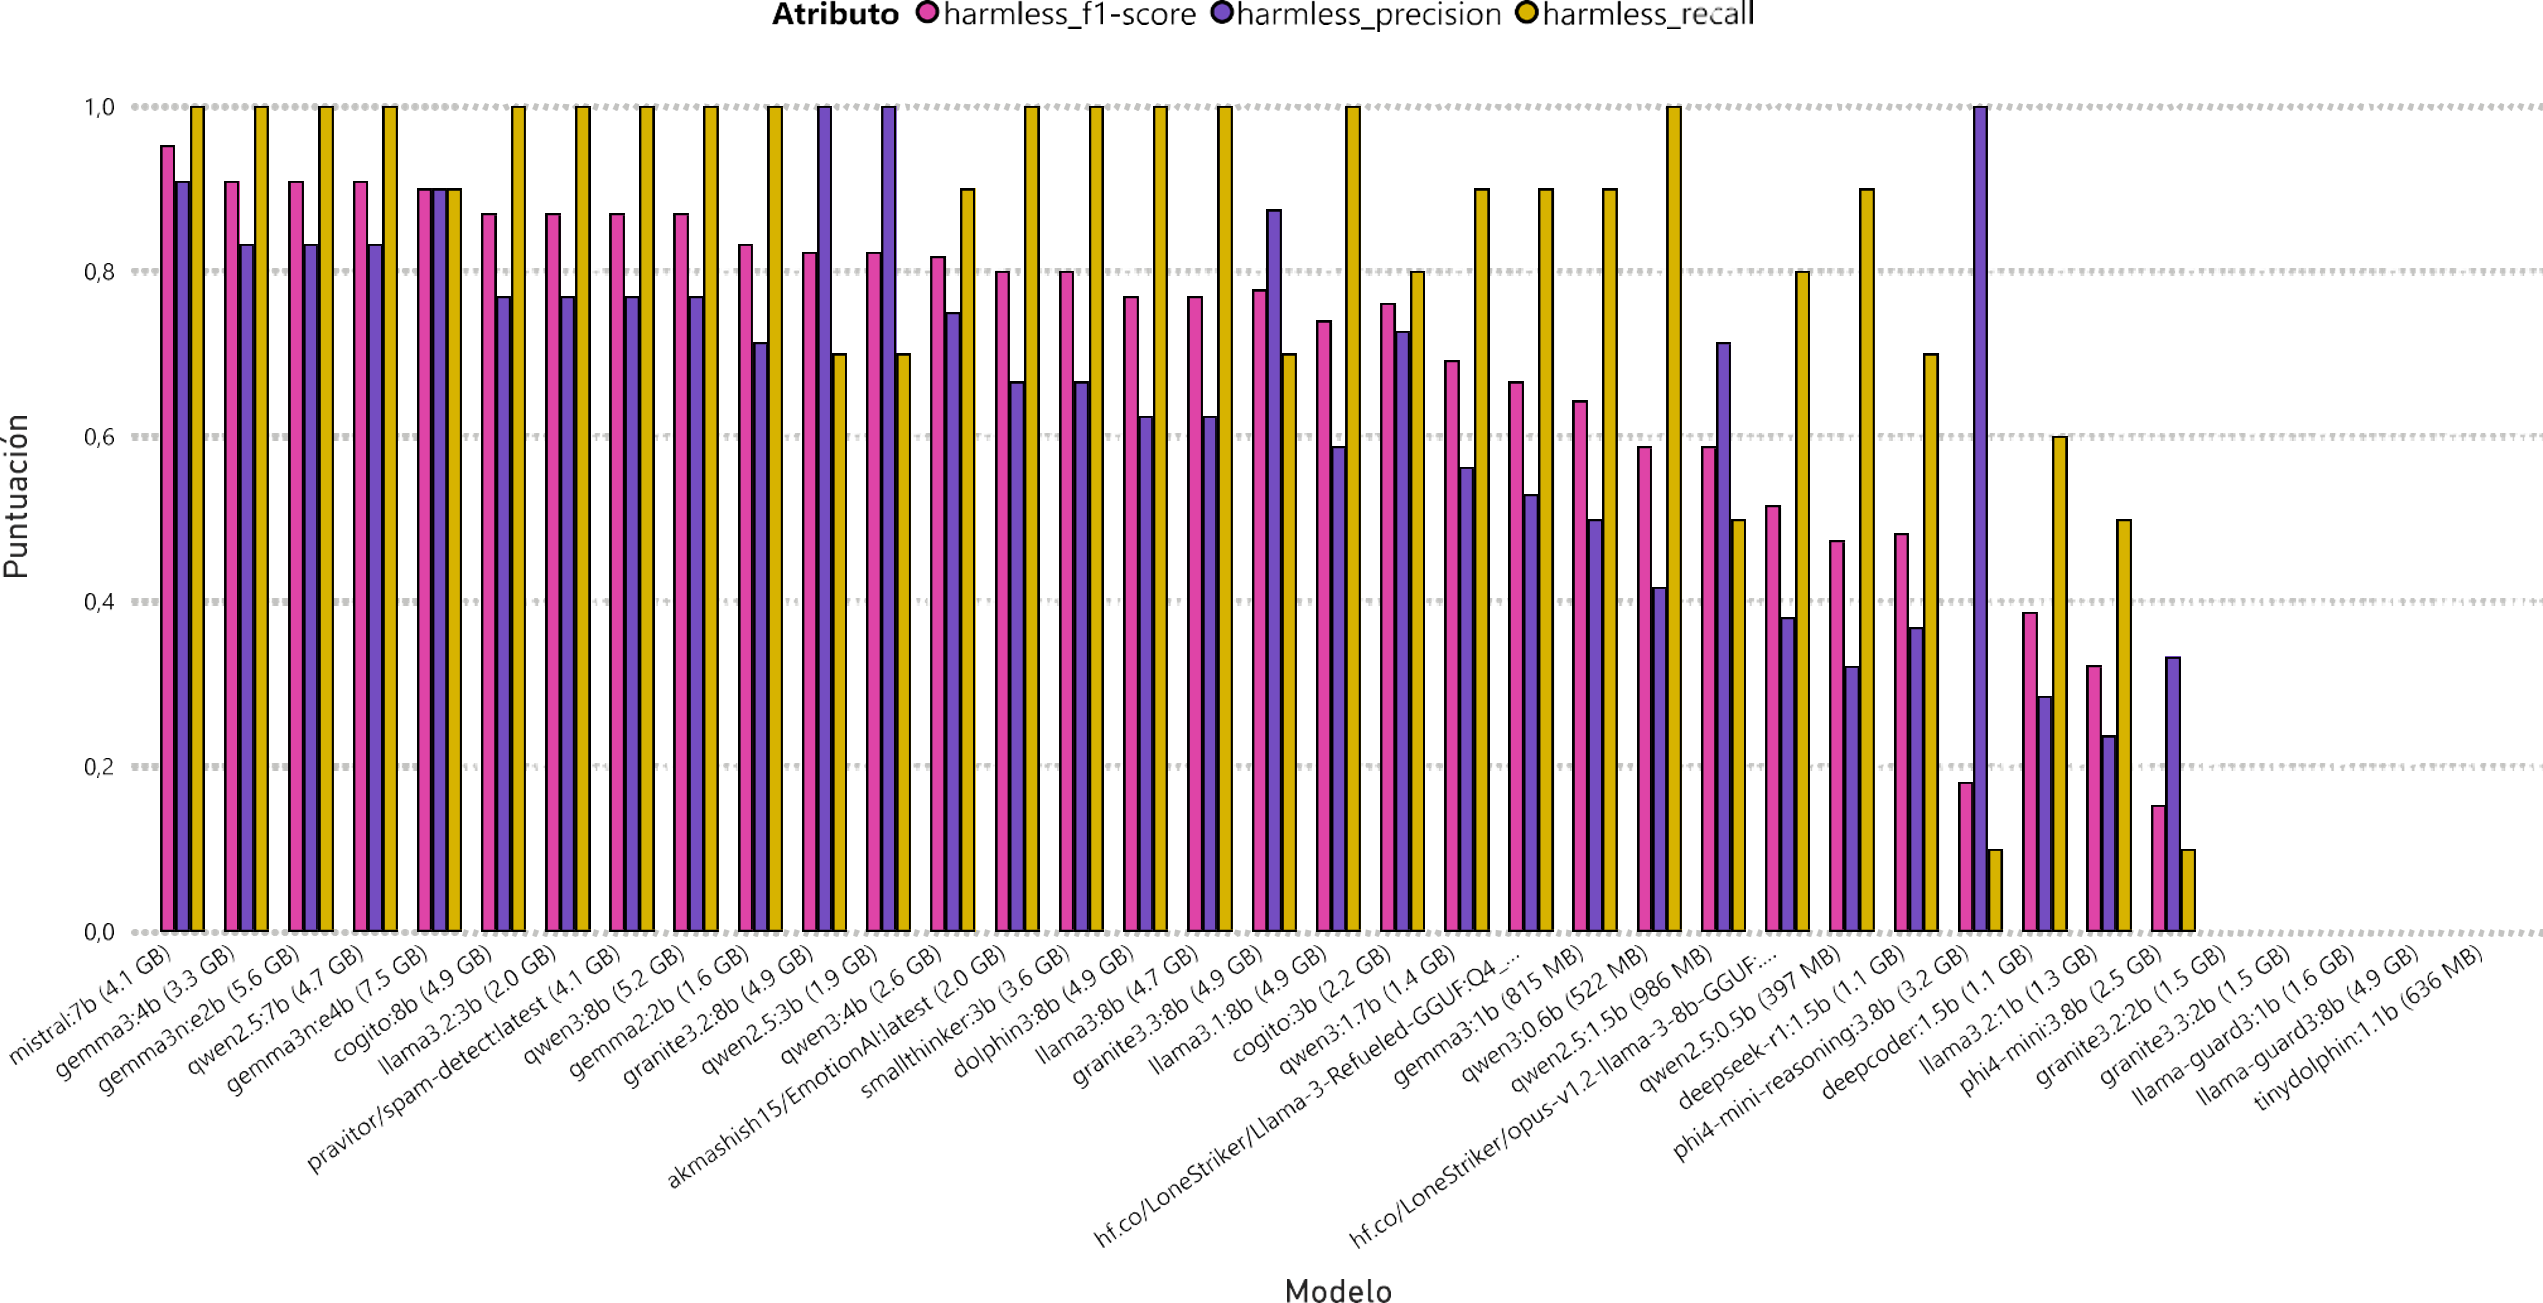
\includegraphics[width=1\linewidth]{imagenes/classificationTestsResults/Few Shot Real Inofensivo.png}
    \caption{Resultados de las pruebas de identificación de inofensivo con la técnica Few Shot prompting a partir de un data set de refinamiento construido con datos reales}
    \label{fig:few-shot-real-inofensivo}
\end{figure}

%28-06-2025: analisis de resultados: se puede decir que se pudieron identificar mensajes relacionados con catfishing y que estas pueden ser el factor inicial pero que habria que vincularlo con un proceso de cadena de custodia para proporcionarlo en un ambiente legal, lo de la hipotesis 2 por tanto podria quedar en analisis de resultados y conclusiones referenciandola como otra posible problematica a atacar a futuro con colaboracion de la mano de perfiles relacionados al area legal que proporcionen expertiz en la cadena de custodia
